
\chapter{Grothendieck \topos{}与空间的概念}

\philoquote{
	Le point de vue et le langage des faisceaux introduit par Leray nous a amené à regarder les ``espaces'' et ``variétés'' en tous genres dans une lumière nouvelle.
	Ils ne touchaient pas, pourtant, à la notion même d'espace, se contentant de nous faire appréhender plus finement, avec des yeux nouveaux, ces traditionnels ``espaces'',
	déjà familiers à tous.
	
	~\\
	
	%Or, il s'est avéré que cette notion d'espace est inadéquate pour rendre compte des ``invariants topologiques'' les plus essentiels qui expriment la ``forme'' des variétés algébriques ``abstraites'' (comme celles auxquelles s'appliquent les conjectures de Weil), voire celle des ``schémas'' généraux (généralisant les anciennes variétés).
	\quad[C]e qui compte vraiment dans un espace topologique, ce ne sont nullement ses ``points'' ou ses sous-ensembles de points, et les relations de proximité etc entre ceux-ci, mais que ce sont les faisceaux sur cet espace, et la catégorie qu'ils forment.
	}{Grothendieck, Récoltes et Semailles\footnotemark}
\footnotetext{这两段评注出自 Grothendieck 的自传 ``收获与播种''.
	
Leray 引入的层的观点和语言使我们以新的视角看待各种 ``空间'' 和 ``流形''. 然而, 它们并未触及空间的概念本身, 只是用新的眼光更加精细地理解那些传统的, 人们早已熟知的空间. % 然而, 事实证明, 这种空间的概念无法准确表达 ``抽象'' 代数簇 (如 Weil 猜想所使用的代数簇) 以及 (推广了传统代数簇的) 一般的 ``概形'' 最本质的 ``拓扑不变量''.

拓扑空间中真正重要的不是它的 ``点'' 或点集的子集, 以及点之间的邻近关系等等, 而是这个空间上的层, 以及它们构成的范畴.
}

\label{chapter-grothendieck-toposes}

\minitoc

\topos{}的概念最早由 Grothendieck 提出. 他将其命名为 topos\footnote{希腊文, ``位置''}, 意在表达这个概念是能够承载拓扑与几何直观的最广泛的概念.

拓扑空间 $X$ 上的层构成一个\topos{} $\operatorname{Sh}(X)$, 称为\emph{层\topos{}} (sheaf topos). 这个\topos{}很大程度上反映了空间 $X$ 的信息. Grothendieck 将层的概念由拓扑空间推广到了最一般的语境, 由此得到一种极为广泛的空间概念; 他将其命名为\emph{景} (site). 景上的层构成的范畴即是所谓 \emph{Grothendieck \topos{}}.

Grothendieck 的想法是, 一个\topos{}不一定来自普通的拓扑空间, 但由于它与 (拓扑空间上的) 层范畴极为相似的性质, 我们可以设想它是一个假想的空间上的层范畴, 即其中的对象是这个假想的空间之上的层. 这个想法也可视为代数--几何对偶的一例: 正如 Gelfand 考虑 Hausdorff 空间上的复值连续函数, Grothendieck 考虑空间上的 ``集合值连续函数''.

% 层\topos{}中的真值是 $X$ 的一个开集, 代表命题 ``在 $X$ 上的何处成立''. 从外部看, $X$ 上的层可视为沿着 $X$ ``一族连续变化的对象'', 而在层\topos{}的语言中, 一个层仿佛单个的对象.

% 这几句话放这里不合适. 该放哪里?

我们从层的一般概念讲起.

\section{预层}

%\subsection{范畴上的预层}

\begin{definition}{(小范畴上的预层)}
    设 $\mathsf C$ 是小范畴. 定义 $\mathsf C$ 上的\emph{预层} (presheaf) 是 $\mathsf C^{\op}$ 到 $\mathsf {Set}$ 的函子.
    记 $\mathsf C$ 上的预层范畴为 $\widehat {\mathsf C} := \mathsf {Fun}(\mathsf C^{\op},\mathsf {Set})$.
\end{definition}

\begin{remark}
	[label={remark-probe}]
	{(预层的一种重要观点)}
	设 $\mathsf C$ 为一系列熟悉的几何对象组成的范畴, 如单纯形 (例 \ref{Simplicial-Sets}), 欧氏空间 (例 \ref{cartsp-site}).
	想象一个未知的空间 $F$, 我们了解这个空间仅有的手段就是用 $\mathsf C$ 的对象 $c$ 来\emph{探测} (probe), 即考虑态射 ``$c\to F$''. 记 $F(c)$ 为所有态射 ``$c\to F$'' 的集合, 那么态射 $d\to c$ 与态射 ``$c\to F$'' 应当可以复合为 $d\to c\to F$, 给出集合的映射 $F(c) \to F(d)$. 这便是预层 $F \colon \mathsf C^{\op} \to \mathsf {Set}$.
	由米田引理,
	态射 ``$c\to F$'' 可赋予真实的含义, 它就是态射 (自然变换) $\yo(c)\to F$.
	在后文中, 我们将不再区分态射 $\yo(c)\to F$ 与 $F(c)$ 的元素.
\end{remark}

%由 $\mathsf C$ 的对象 $c$, 可得 $\mathsf C$ 上的预层 $\operatorname{Hom}_{\mathsf C}(-,c)$. 这事实上是 $\mathsf C$ 到 $\widehat {\mathsf C}$ 的嵌入.
%\begin{definition}
%    {(米田嵌入)}
%    小范畴 $\mathsf C$ 的\emph{米田嵌入}是指函子
%    $\yo\colon \mathsf C \to \widehat{\mathsf C}$,
%    $c\mapsto \yo(c) = \operatorname{Hom}_{\mathsf C}(-,c)$. 米田嵌入的像 $\yo(c)$ 称为\emph{可表函子} (representable functor).
%\end{definition}
%
%\begin{remark}{}
%    米田嵌入也可定义为函子 $\operatorname{Hom}\colon \mathsf C^{\op}\times\mathsf C \to \mathsf {Set}$ 对应的函子
%    $\mathsf C \to \mathsf {Fun}(\mathsf C^{\op},\mathsf {Set})$. 这是因为 $\widehat {\mathsf {C}}$ 是 ``范畴的范畴'' 中的指数对象.
%\end{remark}
%
%这样一个自然变换由 $\operatorname{id}_c \in \yo(c)(c)$ 的像 ($F(c)$ 的元素) 唯一决定, 因此有如下的结论.
%\begin{prop}{(米田引理)}
%    对任意 $F \in \widehat {\mathsf C}$, 有自然同构
%    $$
%    \operatorname{Hom}_{\widehat {\mathsf C}}(\yo(c),F) \simeq F(c).
%    $$
%\end{prop}
%
%\begin{remark}{}
%    米田引理在逻辑上是平凡的; 它带给我们的\emph{观点}, 即 $\mathsf C$ 的对象 $c$ 可\emph{等同于}函子 $\yo(c)$, 比命题本身更重要. 后面我们将大量使用这种观点.
%
%    关于米田引理的更多应用, 以及预层范畴的更多性质, 见附录 \ref{yoneda} 节.
%\end{remark}

范畴上预层的概念来自拓扑空间上的预层.
设 $X$ 为拓扑空间, 记 $\operatorname{Open}(X)$ 为 $X$ 的开集在包含关系下构成的范畴.

\begin{definition}
	{(拓扑空间上的预层)}
	拓扑空间 $X$ 上的\emph{预层}是 $\operatorname{Open}(X)$ 上的预层, 也即函子 $\operatorname{Open}(X)^{\op} \to \mathsf {Set}$.
	记 $X$ 上的预层范畴为 $\operatorname{Presh}(X)$.
\end{definition}

\begin{remark}
	{}
	需要注意的一点是, 拓扑空间 $X$ 到范畴 $\operatorname{Open}(X)$ 的对应是反变的, 也即对连续映射 $f\colon X \to Y$, 我们有反方向的函子 $f^{-1}\colon \operatorname{Open}(Y) \to \operatorname{Open}(X)$, 将开子集 $U\subset Y$ 对应到 $f^{-1}(U)\subset X$.
	这也是一种代数--几何对偶.
\end{remark}

\subsection{常见的预层范畴}

\begin{example}
    {(集合)}
    记 $\mathsf {1}$ 为仅有一个对象和一个态射的范畴.
    $\mathsf {1}$ 上的预层范畴 $\widehat {\mathsf 1} = \mathsf {Set}^{\mathsf {1}^\op}$ 等同于集合范畴 $\mathsf {Set}$.
    它也可视为单点空间上的层范畴;
    它在\topos{}中扮演的角色等同于一个点在拓扑空间中扮演的角色.
\end{example}

\begin{example}
    [label={Simplicial-Sets}]
    {(单纯集)}
    令范畴 $\Delta$ 为有限全序集 $[0],[1],[2],\cdots$ 与保序映射构成的范畴, 其中 $[n] = \{0,1,\cdots,n\}$, 称映射 $f \colon [n] \to [m]$ 为保序映射是指当 $i\leq j$ 时 $f(i)\leq f(j)$.
    我们将 $[n]$ 想象为 $n$ 维单纯形.
    称范畴 $\Delta$ 为\emph{单纯范畴} (simplicial category).

    $\Delta$ 上的预层称为\emph{单纯集} (simplicial set), 也就是可用单纯形来探测的空间. 记单纯集范畴为
    $\mathsf {sSet}=\widehat {\Delta}=\mathsf {Fun}(\Delta^{\op},\mathsf {Set})$.
    
    对于单纯集 $X \colon 
    \Delta^{\op} \to \mathsf {Set}$,
    $X([n])$ 表示 $X$ 中 $n$ 维单形的集合,
    其中含有退化的单形.
    记米田嵌入 $\yo([n])$ 为 $\Delta^n$,
    米田引理告诉我们
    $$
    X([n]) \simeq \operatorname{Hom}_{\mathsf {sSet}}(\Delta^n,X),
    $$
    因此如上关于 $X([n])$ 的解释是准确的.
\end{example}

\begin{example}
    {(有向图)}
    有向图可用类似于单纯集 (例 \ref{Simplicial-Sets}) 的方式定义.
    考虑范畴
    $$
    \mathsf C=
    \Big\{\!
    \begin{tikzcd}[ampersand replacement=\&]
	{[0]} \& {[1]}
	\arrow["s", shift left, from=1-1, to=1-2]
	\arrow["t"', shift right, from=1-1, to=1-2]
    \end{tikzcd}
    \!\Big\},
    $$
    其中 $s,t\colon [0]\to [1]$
    分别将 $0\in [0]$ 映射到 $0\in [1]$ 和 $1\in [1]$.
    那么 $\mathsf C$ 上的预层 $X\colon \mathsf C^{\op}\to\mathsf {Set}$ 可视为有向图:
    $X([0])$ 是有向图的顶点集, $X([1])$ 是有向图的边集;
    映射 $X(s),X(t)\colon X([1])\to X([0])$ 将有向图的边对应到其起点与终点.
\end{example}

\begin{example}
    [label={G-set-presheaf-category}]
    {($G$-集)}
    设 $G$ 是群. 定义范畴 $\mathsf BG$ 为仅有一个对象的范畴,
    这个对象到自身的态射集为 $G$.
    $\mathsf BG$ 上的预层是函子 $(\mathsf B G)^{\op} \simeq \mathsf B(G^{\op}) \to \mathsf {Set}$, 等同于具有 $G^{\op}$-左作用即 $G$-右作用的集合, 也称为 $G$-集或 $G$ 的表示. 记 $G$-集的范畴为 $G\mathsf {Set}$.
\end{example}

%\subsection{拓扑空间上的预层}

\subsection{预层范畴是\topos{}}

下面我们说明小范畴 $\mathsf C$ 上的预层范畴 $\widehat {\mathsf C}$ 是一个\topos{}.

\begin{prop}
	[label={presheaf-category-complete}]
	{(预层范畴完备且余完备)}
    $\widehat {\mathsf C}$ 是\emph{完备} (complete) 且\emph{余完备} (cocomplete) 的, 也即具有一切 (小) 极限与余极限.
\end{prop}

\begin{proof}
    预层的极限可 ``逐点'' 计算: 设 $F \colon I \to \widehat {\mathsf C}, i \mapsto F_i$ 是任意图表, 那么其极限为
    $$
    \big({\lim_I F_i}\big)(c) = \lim_I F_i(c),
    $$
    余极限类似.
\end{proof}

特别地, 预层范畴 $\widehat {\mathsf C}$ 的终对象 (空图的极限) 是将所有对象 $c$ 对应到 $\mathsf {Set}$ 的终对象 $1$ 的预层, 而始对象 (空图的余极限) 将所有对象对应到 $\mathsf {Set}$ 的始对象 $\varnothing$.
预层的积与和即是逐点的积与和.

\begin{prop}
	[label={presheaf-category-exponential}]
	{}
    $\widehat{\mathsf C}$ 是积闭范畴.
\end{prop}

\begin{proof}
    对 $X,Y \in \widehat {\mathsf C}$,
    我们不能以 $Y^X(c) = Y(c)^{X(c)}$ 来定义指数对象 $Y^X$, 因为这个构造没有函子性.
    一种可行的思路如下. 假设指数对象 $Y^X$ 存在, 即有 (关于 $Z$ 的) 自然同构
    $$
    \operatorname{Hom}_{\widehat{\mathsf C}}(Z,Y^X) \simeq \operatorname{Hom}_{\widehat{\mathsf C}}(Z\times X,Y).
    $$
    代入 $Z=\yo(c)$, 由米田引理便得到 (关于 $c$ 的) 自然同构
    $$
    Y^X(c) = \operatorname{Hom}_{\widehat{\mathsf C}}(\yo(c)\times X,Y),
    $$
    这已经确定了函子 $Y^X$.
    对任意 $Z\in \widehat {\mathsf C}$,
    将其表示为可表函子的余极限
    $Z = \operatorname{colim}_{\yo(c)\to Z}\yo(c)$ (命题 \ref{presheaf-as-colimit-of-representables}),
    那么
    \[
    \begin{aligned}
    	\operatorname{Hom}_{\widehat {\mathsf C}}(Z,Y^X)&\simeq
    	\operatorname{lim}_{\yo(c)\to Z}\operatorname{Hom}_{\widehat{\mathsf C}}(\yo(c),Y^X)\\&\simeq
    	\operatorname{lim}_{\yo(c)\to Z}\operatorname{Hom}_{\widehat{\mathsf C}}(\yo(c)\times X,Y)\\&\simeq
    	\operatorname{Hom}_{\widehat{\mathsf C}}(\operatorname{colim}_{\yo(c)\to Z}(\yo(c)\times X),Y)\\&\simeq
    	\operatorname{Hom}_{\widehat{\mathsf C}}(Z\times X,Y).
	\end{aligned}
    \]
%    下面验证这个函子确实满足指数对象的条件.
%
%    首先给出取值映射 $\operatorname{ev} \colon Y^X \times X \to Y$,
%    也即自然的映射
%    $$
%    \operatorname{Hom}_{\widehat C}(\yo(c)\times X,Y)\times X(c)\to Y(c).
%    $$
%    对 $\theta \in \operatorname{Hom}_{\widehat C}(\yo(c)\times X,Y)$,
%    考虑 $\theta_c \colon \yo(c)(c)\times X(c) \to Y(c)$,
%    代入 $\operatorname{id}_c$ 便得到映射 $X(c)\to Y(c)$.
%    
%    \todo{}
	最后一步用到 $-\times X$ 保持余极限, 因为预层的余极限是逐点的.
\end{proof}

由命题 \ref{slice-of-presheaf-is-presheaf-over-slice}, $\widehat {\mathsf C}$ 甚至是局部积闭范畴.

\subsection{筛与预层范畴中的子对象}

本节的目标是描述预层范畴 $\widehat{\mathsf C}$ 中的子对象以及子对象分类子.

\begin{propdef}
    [label={subfunctor-description}]
    {(子函子)}
    $\widehat{\mathsf C}$ 中的态射 $Y \to X$ 是单射, 当且仅当对每个对象 $c$, 映射 $Y(c) \to X(c)$ 都是子集,
    且对每个态射 $c\to d$, 映射 $Y(d) \to Y(c)$ 都是 $X(d) \to X(c)$ 的限制; 此时也称 $Y \to X$ 为\emph{子函子} (subfunctor).
\end{propdef}

\begin{proof}
	由单射的拉回刻画 (命题 \ref{mono-epi-pullback-pushout}) 以及 $\widehat {\mathsf C}$ 中极限的逐点计算 (命题 \ref{presheaf-category-complete}) 即证.
\end{proof}

\emph{筛}的概念可帮助描述预层范畴的子对象分类子.

\begin{definition}
	[label={sieve}]
    {(筛)}
    范畴 $\mathsf C$ 的对象 $c$ 上的一个\emph{筛} (英 sieve, 法 crible) 是指 $\mathsf C$ 中一族指向 $c$ 的箭头 \makebox{$S= \{f \colon d \to c\}$}, 构成 $\mathsf C$ 的\emph{右理想}; 也即对任意 $f\in S$ 与 $\mathsf C$ 中任意箭头 $g$, 只要 $fg$ 可定义, 就有 $fg \in S$.
    
    对于两个筛 $R,S$, 若 $R\subset S$, 则称 $R$ 比 $S$ 更细, 或 $R$ 是 $S$ 的一个\emph{细化} (refinement).
    
    设 $R$ 是一族指向 $c$ 的箭头, 定义 $R$ \emph{生成}的筛为  $\{e\to d\to c\mid (d\to c)\in R \}$, 也即包含 $R$ 中所有箭头的最细的筛.
    
    对于 $\mathsf C$ 中的态射 $f\colon d\to c$ 以及 $c$ 上的筛 $S$, 定义\emph{筛的拉回} $f^*S$ 为
    \[
    f^*S = \{ g\colon e\to d \mid fg\in S \}.
    \]
    当范畴 $\mathsf C$ 中存在拉回时, $f^*S$ 恰好由 $S$ 中所有元素沿 $f$ 的拉回构成.
\end{definition}

\begin{remark}
    {(筛的直观)}
    筛是一种能把大的东西挡住, 让小的东西通过的工具. 想象 $S$ 的元素为可以 ``通过'' $S$ 的箭头.
    若 $d \overset{f}{\longrightarrow} c$ 可以 ``通过'' $S$, 那么 $e \overset{g}{\longrightarrow} d \overset{f}{\longrightarrow} c$ 比 $d \overset{f}{\longrightarrow} c$ ``小'', 从而它也可以 ``通过'' $S$.

    \begin{center}
        

\tikzset{every picture/.style={line width=0.75pt}} %set default line width to 0.75pt        

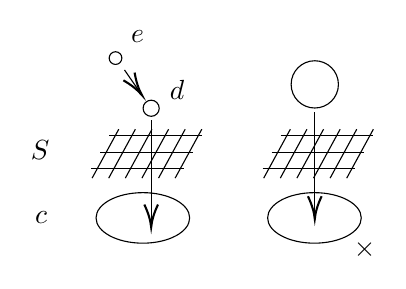
\begin{tikzpicture}[x=0.75pt,y=0.75pt,yscale=-1,xscale=1]
%uncomment if require: \path (0,300); %set diagram left start at 0, and has height of 300

%Shape: Ellipse [id:dp10401378338786049] 
\draw   (74,113.39) .. controls (74,106.67) and (84.1,101.22) .. (96.56,101.22) .. controls (109.01,101.22) and (119.11,106.67) .. (119.11,113.39) .. controls (119.11,120.11) and (109.01,125.56) .. (96.56,125.56) .. controls (84.1,125.56) and (74,120.11) .. (74,113.39) -- cycle ;
%Shape: Grid [id:dp09583060841478219] 
\draw  [draw opacity=0] (81.95,70.67) -- (126.56,70.67) -- (113.72,94.22) -- (69.11,94.22) -- cycle ; \draw   (84.95,70.67) -- (72.11,94.22)(92.95,70.67) -- (80.11,94.22)(100.95,70.67) -- (88.11,94.22)(108.95,70.67) -- (96.11,94.22)(116.95,70.67) -- (104.11,94.22)(124.95,70.67) -- (112.11,94.22) ; \draw   (80.31,73.67) -- (124.92,73.67)(75.95,81.67) -- (120.56,81.67)(71.59,89.67) -- (116.2,89.67) ; \draw    ;
%Shape: Circle [id:dp31189924819685966] 
\draw   (80.33,36.39) .. controls (80.33,34.7) and (81.7,33.33) .. (83.39,33.33) .. controls (85.08,33.33) and (86.44,34.7) .. (86.44,36.39) .. controls (86.44,38.08) and (85.08,39.44) .. (83.39,39.44) .. controls (81.7,39.44) and (80.33,38.08) .. (80.33,36.39) -- cycle ;
%Straight Lines [id:da12935033787340267] 
\draw    (87.72,42.11) -- (94.97,52.58) ;
\draw [shift={(96.11,54.22)}, rotate = 235.29] [color={rgb, 255:red, 0; green, 0; blue, 0 }  ][line width=0.75]    (10.93,-3.29) .. controls (6.95,-1.4) and (3.31,-0.3) .. (0,0) .. controls (3.31,0.3) and (6.95,1.4) .. (10.93,3.29)   ;
%Shape: Circle [id:dp7222065551952845] 
\draw   (96.67,60.56) .. controls (96.67,58.41) and (98.41,56.67) .. (100.56,56.67) .. controls (102.7,56.67) and (104.44,58.41) .. (104.44,60.56) .. controls (104.44,62.7) and (102.7,64.44) .. (100.56,64.44) .. controls (98.41,64.44) and (96.67,62.7) .. (96.67,60.56) -- cycle ;
%Straight Lines [id:da7276461675375434] 
\draw    (100.56,66.44) -- (100.56,115.89) ;
\draw [shift={(100.56,117.89)}, rotate = 270] [color={rgb, 255:red, 0; green, 0; blue, 0 }  ][line width=0.75]    (10.93,-3.29) .. controls (6.95,-1.4) and (3.31,-0.3) .. (0,0) .. controls (3.31,0.3) and (6.95,1.4) .. (10.93,3.29)   ;
%Shape: Ellipse [id:dp12697611260252684] 
\draw   (156.67,113.39) .. controls (156.67,106.67) and (166.77,101.22) .. (179.22,101.22) .. controls (191.68,101.22) and (201.78,106.67) .. (201.78,113.39) .. controls (201.78,120.11) and (191.68,125.56) .. (179.22,125.56) .. controls (166.77,125.56) and (156.67,120.11) .. (156.67,113.39) -- cycle ;
%Shape: Grid [id:dp9936460967678797] 
\draw  [draw opacity=0] (164.61,70.67) -- (209.22,70.67) -- (196.39,94.22) -- (151.78,94.22) -- cycle ; \draw   (167.61,70.67) -- (154.78,94.22)(175.61,70.67) -- (162.78,94.22)(183.61,70.67) -- (170.78,94.22)(191.61,70.67) -- (178.78,94.22)(199.61,70.67) -- (186.78,94.22)(207.61,70.67) -- (194.78,94.22) ; \draw   (162.98,73.67) -- (207.59,73.67)(158.62,81.67) -- (203.23,81.67)(154.26,89.67) -- (198.87,89.67) ; \draw    ;
%Shape: Circle [id:dp838751100400853] 
\draw   (168,49.06) .. controls (168,42.77) and (173.1,37.67) .. (179.39,37.67) .. controls (185.68,37.67) and (190.78,42.77) .. (190.78,49.06) .. controls (190.78,55.35) and (185.68,60.44) .. (179.39,60.44) .. controls (173.1,60.44) and (168,55.35) .. (168,49.06) -- cycle ;
%Straight Lines [id:da5932706956135338] 
\draw    (179.39,62.44) -- (179.39,111.89) ;
\draw [shift={(179.39,113.89)}, rotate = 270] [color={rgb, 255:red, 0; green, 0; blue, 0 }  ][line width=0.75]    (10.93,-3.29) .. controls (6.95,-1.4) and (3.31,-0.3) .. (0,0) .. controls (3.31,0.3) and (6.95,1.4) .. (10.93,3.29)   ;

% Text Node
\draw (43.33,109) node [anchor=north west][inner sep=0.75pt]   [align=left] {$\displaystyle c$};
% Text Node
\draw (41.33,75) node [anchor=north west][inner sep=0.75pt]   [align=left] {$\displaystyle S$};
% Text Node
\draw (113,123.67) node [anchor=north west][inner sep=0.75pt]   [align=left] {$\displaystyle \checkmark$};
% Text Node
\draw (197,123) node [anchor=north west][inner sep=0.75pt]   [align=left] {$\displaystyle \times $};
% Text Node
\draw (108.33,46) node [anchor=north west][inner sep=0.75pt]   [align=left] {$\displaystyle d$};
% Text Node
\draw (89.67,22) node [anchor=north west][inner sep=0.75pt]   [align=left] {$\displaystyle e$};


\end{tikzpicture}
    \end{center}

    % 这里, 我们认为指向 $c$ 的态射越复合就越小. 回忆环是一个对象的 $\mathsf {Ab}$-充实范畴, 那么其中的筛正是环的右理想; 筛的大小观念类似于 $p$-进度量下的整数越乘越小.

    一个筛越细, 能 ``通过'' 它的东西就越少, 这解释了\emph{细化}的含义; 反之, 所有东西都能通过的筛就是最粗的筛.
\end{remark}

\begin{example}
	[label={sieve-from-cover}]
	{(覆盖产生筛)}
	设 $X$ 为拓扑空间, $\{U_i\}$ 是其中开集 $V$ 的一个开覆盖. 那么
	$$
	\big\{W\subset V \mid \exists i, W \subset U_i\big\}
	$$
	构成 $\operatorname{Open}(X)$ 中 $V$ 上的一个筛. 直观上每个 $U_i$ 是筛上的一个 ``洞'', 比它小的对象能 ``通过'' 这个筛.
\end{example}

\begin{prop}
	[label={sieve-and-subfunctor}]
    {(筛与子函子)}
    范畴 $\mathsf C$ 的对象 $c$ 上的筛自然地一一对应于 $\yo(c)$ 的子函子.
\end{prop}

\begin{proof}
    设 $S$ 是 $c$ 上的筛, 那么
    $$
    X\colon \mathsf C^{\op}\to\mathsf {Set},\,X(d) := \{f\colon d\to c \mid f\in S\} \subset \operatorname{Hom}_{\mathsf C}(d,c) = \yo(c)(d)
    $$
    构成 $\yo(c)$ 的子函子.
    设 $X \to \yo(c)$ 为子函子, 那么
    $$
    S:=\big\{
        f \colon d\to c \mid f\in X(d)
    \big\}
    $$
    是 $c$ 上的筛. 很明显, 这两个对应是互逆的.
    注意 $X$ 的函子性恰好等价于筛 $S$ 为右理想.
    容易验证筛 $S$ 沿态射 $f\colon d\to c$ 的拉回等同于 $\yo(c)$ 的子对象 $X$ 沿 $f$ 的拉回.
\end{proof}

在后文中, 我们将自由地运用上述对应, 将 $c$ 上的筛与 $\yo(c)$ 的子函子完全等同, 请读者务必熟悉.

%\begin{remark}
%    {}
%    若将 $\widehat {\mathsf C}$ 的对象称作 $\mathsf C$ 的 ``广义对象'', 那么 $\yo(c)$ 的子函子可称作 $c$ 的 ``广义子对象''.
%
%    $\mathsf C$ 的 ``广义对象'' $X$ 的子对象, 根据命题 \ref{subfunctor-description} 的描述, 也可视为 $X$ 上的 ``筛''.
%\end{remark}

\begin{example}
	[label={principal-sieve}]
	{(主筛)}
	对于范畴 $\mathsf C$ 中的态射 $f\colon c'\to c$,
	所有穿过 $f$ 的态射 $c''\to c'\overset{f}{\to} c$ 构成 $c$ 上的一个筛 $\downarrow f$, 称为\emph{主筛} (principal sieve).
	这类似于环的主理想.
	$\downarrow f$ 对应的 $\yo(c)$ 的子函子恰为 $\yo(f)\colon \yo(c') \to \yo(c)$ 的像.
\end{example}

\begin{example}
	[label={sieve-from-cover-subfunctor}]
	{(覆盖产生的筛对应的子函子)}
	继续例 \ref{sieve-from-cover}, 设 $S$ 为覆盖 $\{U_i\}$ 生成的筛 (视为 $\yo(V)$ 的子函子), 那么下图是余等化子.
	\begin{equation}
		\label{sieve-coeq}
		\begin{tikzcd}[ampersand replacement=\&]
			{\coprod_{i,j}\yo(U_i\cap U_j)} \& {\coprod_i \yo(U_i)} \& S
			\arrow[shift right, from=1-1, to=1-2]
			\arrow[shift left, from=1-1, to=1-2]
			\arrow[from=1-2, to=1-3]
		\end{tikzcd}
	\end{equation}
	这是因为, 由 $S$ 的定义, 对 $W\in\operatorname{Open}(X)$, 若存在 $i$, $W\subset U_i$, 则 $S(W)$ 是单元集; 否则 $S(W)$ 是空集. 由此可知下图是集合范畴中的余等化子.
	\[\begin{tikzcd}[ampersand replacement=\&, column sep=small]
		{\coprod_{i,j}\operatorname{Hom}_{\operatorname{Open}(X)}(W,U_i\cap U_j)} \& {\coprod_i \operatorname{Hom}_{\operatorname{Open}(X)}(W,U_i)} \& {S(W)}
		\arrow[shift right, from=1-1, to=1-2]
		\arrow[shift left, from=1-1, to=1-2]
		\arrow[from=1-2, to=1-3]
	\end{tikzcd}\]
	而预层的余极限是 ``逐点'' 的, 于是得 (\ref{sieve-coeq}).
	
	对 $X$ 上的任意预层 $F$, 以 $\operatorname{Hom}_{\operatorname{Presh}(X)}(-,F)$ 作用于 (\ref{sieve-coeq}), 可知下图是集合范畴中的等化子.
	\begin{equation}
		\begin{tikzcd}[ampersand replacement=\&]
			{\operatorname{Hom}_{\operatorname{Presh}(X)}(S,F)} \& {\prod_i F(U_i)} \& {\prod_{i,j}F(U_i\cap U_j)}
			\arrow[shift left, from=1-2, to=1-3]
			\arrow[shift right, from=1-2, to=1-3]
			\arrow[from=1-1, to=1-2]
		\end{tikzcd}
		\label{sieve-subfunctor-equalizer}
	\end{equation}
	因此态射集合 $\operatorname{Hom}_{\operatorname{Presh}(X)}(S,F)$ 表达了预层 $F$ 关于覆盖 $\{U_i\}$ 的下降资料 (descent data), 由覆盖 $\{U_i\}$ ``下降'' 到 $V$. 若 $F$ 为层, 就应该有 $$\operatorname{Hom}_{\operatorname{Presh}(X)}(S,F) \simeq F(V) \simeq \operatorname{Hom}_{\operatorname{Presh}(X)}(\yo(V),F).$$
\end{example}

\begin{example}
	[label={maximal-sieve}]
    {(极大筛)}
    所有指向 $c$ 的箭头的集合称为\emph{极大筛}, 也即最粗的筛.
    它对应 $\yo(c)$ 的子对象 $\yo(c)$ 自身.
    注意, $c$ 上的一个筛是极大筛当且仅当它包含 $\operatorname{id}_c$.
    设 $S$ 是 $c$ 上的筛, $f\colon d\to c$, 那么 $f\in S$ 当且仅当 $f^*S$ 为 $d$ 上的极大筛.
\end{example}

假设 $\widehat{\mathsf C}$ 中存在子对象分类子 $\Omega$, 那么由米田引理, 有自然同构
$$
\Omega(c) \simeq \operatorname{Hom}_{\widehat {\mathsf C}}(\yo(c),\Omega)
\simeq \operatorname{Sub}_{\widehat {\mathsf C}}(\yo(c))\simeq \{\text{$c$ 上的筛}\}.
$$
\begin{prop}
	[label={presheaf-category-subobject-classifier}]
	{(预层范畴的子对象分类子)}
	在任意范畴 $\mathsf C$ 上, 定义预层 $\Omega\colon \mathsf C^{\op}\to\mathsf {Set}$, $\Omega(c) := \{\text{$c$ 上的筛}\}$, 且对态射 $f\colon d\to c$, $\Omega(f)\colon \Omega(c)\to \Omega(d)$ 为筛的拉回. 那么 $\Omega$ 是 $\widehat{\mathsf C}$ 的子对象分类子.
\end{prop}

\begin{proof}
    定义态射 $\top\colon 1 \to \Omega,$
    对每个对象 $c$ 选出 $\Omega(c)= \operatorname{Sub}_{\widehat {\mathsf C}}(\yo(c))$
    中的子对象 $\yo(c)$ 自身, 也即 $c$ 上的极大筛.
    设 $Y\to X$ 是 $\widehat{\mathsf C}$ 中的任意子对象.
    定义态射 $\chi \colon X \to \Omega$, 将 $x\in X(c)$ 对应到 $c$ 上的筛
    $$
    \chi_c(x) := \big\{f \colon d \to c \mid X(f)(x) \in Y(d)\big\}.
    $$
    注意 $\chi_c(x)$ 是极大筛当且仅当 $\operatorname{id}_c \in \chi_c(x)$, 也即 $x \in Y(c)$,
    所以子对象 $Y\to X$ 是如下的拉回.
    % https://q.uiver.app/#q=WzAsNCxbMCwxLCJYIl0sWzEsMSwiXFxPbWVnYSJdLFsxLDAsIjEiXSxbMCwwLCJZIl0sWzMsMF0sWzAsMSwiXFxjaGkiLDJdLFsyLDEsIlxcdG9wIl0sWzMsMl1d
    \[\begin{tikzcd}[ampersand replacement=\&]
    	Y \& 1 \\
    	X \& \Omega
    	\arrow[from=1-1, to=2-1]
    	\arrow["\chi"', from=2-1, to=2-2]
    	\arrow["\top", from=1-2, to=2-2]
    	\arrow[from=1-1, to=1-2]
    \end{tikzcd}\]
	这证明了 $\Omega$ 是 $\widehat{\mathsf C}$ 的子对象分类子, 且 $\top\colon 1\to\Omega$ 是万有子对象.
\end{proof}

\begin{remark}{}
	上面给出的态射 $X\to\Omega$ 的构造并非空中楼阁.
	事实上, 假设下图中右侧方块以及长方形为拉回,
	可得左侧方块为拉回,
	% https://q.uiver.app/#q=WzAsNixbMSwwLCJZIl0sWzEsMSwiWCJdLFswLDEsIlxceW8oYykiXSxbMiwwLCIxIl0sWzIsMSwiXFxPbWVnYSJdLFswLDAsIlxcY2hpX2MoeCkiXSxbMyw0LCJcXHRvcCJdLFsxLDQsIlxcY2hpIiwyXSxbMCwzXSxbMCwxXSxbMiwxLCJ4IiwyXSxbNSwyXSxbNSwwXV0=
	\[\begin{tikzcd}[ampersand replacement=\&]
		{\chi_c(x)} \& Y \& 1 \\
		{\yo(c)} \& X \& \Omega
		\arrow["\top", from=1-3, to=2-3]
		\arrow["\chi"', from=2-2, to=2-3]
		\arrow[from=1-2, to=1-3]
		\arrow[from=1-2, to=2-2]
		\arrow["x"', from=2-1, to=2-2]
		\arrow[from=1-1, to=2-1]
		\arrow[from=1-1, to=1-2]
	\end{tikzcd}\]
	因此 $\chi_c(x) = \{f\in\yo(c)(d)\mid x\circ f\in Y(d)\}$.
	注意到对于 $x\in X(c)$, 有 $x\in Y(c)$ 当且仅当上图中存在提升 $\yo(c)\to Y$,
	当且仅当 $\chi_c(x) = \yo(c)$.
\end{remark}

综合上述论证, 我们得到
\begin{prop}{}
    $\widehat {\mathsf C}$ 是一个\topos{}.
\end{prop}

\begin{example}
    {($G$-集)}
    例 \ref{G-set-presheaf-category} 介绍了 $G$-集范畴, 即 $\mathsf BG$ 上的预层范畴. 由于 $\mathsf BG$ 只有一个对象且态射均为自同构,
    其上仅有两个筛, 空集与极大筛.
    
    因此, $G$-集范畴的子对象分类子 $\Omega$ 是二元集合 $\{\top,\bot\}$, 其上带有 $G$ 的平凡作用.
    事实上, 一个 $G$-集 $X$ 的子对象 $Y$ 是其中 $G$-作用下封闭的子集. 其对应的特征函数 $X\to\{\top,\bot\}$ 就是子集 $Y$ 的特征函数.
\end{example}


\section{景}



Grothendieck 意识到, 层的概念所需的关键信息是一个对象 $U$ 何时被一族进入 $U$ 的态射 (甚至不一定是 $U$ 的子对象) 所\emph{覆盖}.

\subsection{从覆盖到 Grothendieck 拓扑}

本小节有许多的定义, 在读者看来这些定义可能有些冗余. 这或许是历史的遗留, 但每个定义有各自的长处.

\begin{definition}{(覆盖结构)}
    设范畴 $\mathsf C$ 具有拉回.
    $\mathsf C$ 上的一个\emph{覆盖结构} (coverage) $T$ 是如下结构: 对每个对象 $c$ 指定一个集合 $T(c)$, 其元素为态射族 $\{f_i \colon c_i \to c\}_{i\in I}$, 称为 $c$ 的 $T$-\emph{覆盖族} (covering family), 满足
    \begin{itemize}
    	\item (拉回下的稳定性) 若 $\{f_i \colon c_i \to c\}_{i\in I}\in T(c)$, $g \colon d \to c$,
    	则 $\{g^*(f_i) \colon d_i \to d\}_{i\in I}\in T(d)$.
    \end{itemize}
        
    %带有覆盖结构的范畴 $(\mathsf C,T)$ 称为\emph{景} (site).
    对于两个覆盖结构 $T,T'$, 若 $T$-覆盖族都是 $T'$-覆盖族, 则称 $T'$ 较\emph{细} (fine).
\end{definition}

对于拓扑空间的开集范畴, 拉回下的稳定性相当于若一族开集覆盖了 $U$, 那么它们也覆盖了 $U$ 的任何子集.

\begin{remark}
    {}
    当 $\mathsf C$ 不存在拉回时, ``拉回下的稳定性'' 可改为: 若 $\{f_i \colon c_i \to c\}_{i\in I}\in T(c)$, $g \colon d \to c$,
    则存在 $\{h_j \colon d_j \to d\}_{j\in J}\in T(d)$,
    使得每个 $gh_j$ 都穿过某个 $f_i$.
\end{remark}

%\begin{remark}{}
%    上面定义的覆盖结构有时也称为范畴上的 \emph{Grothendieck 拓扑}, 但这个词的含义有时要窄一些.
%\end{remark}

\begin{definition}
	[label={sheaf-condition}]
	{(关于态射族的层条件)}
	
	设 $F$ 是范畴 $\mathsf C$ 上的预层. 设 $M = \{f_i\colon c_i\to c\}_{i\in I}$ 是 $\mathsf C$ 中的一族态射. 称 $F$ 满足关于 $M$ 的\emph{层条件}, 是指对任意一组相容的元素 $(s_i\in F(c_i))_{i\in I}$,
	存在唯一的 $s\in F(c)$ 满足 $$F(f_i)(s)=s_i\,\forall i\in I.$$
	其中, 一组元素 $(s_i\in F(c_i))_{i\in I}$ \emph{相容}是指对任意态射 $f\colon d \to c_i$, $g\colon d \to c_j$, 有 $$F(f)(s_i) = F(g)(s_j) \in F(d).$$
	
	若将上面的 ``存在唯一'' 改为 ``存在至多一个'', 得到的条件称为\emph{分离性}条件.
	
	在 $\mathsf C$ 具有拉回的条件下, 层条件可简洁地表述为如下等化子,
	% https://q.uiver.app/#q=WzAsMyxbMCwwLCJGKGMpIl0sWzEsMCwiXFxwcm9kX3tpfSBGKGNfaSkiXSxbMiwwLCJcXHByb2Rfe2ksan0gRihjX2lcXHRpbWVzX2MgY19qKSJdLFsxLDIsIiIsMCx7Im9mZnNldCI6LTF9XSxbMSwyLCIiLDIseyJvZmZzZXQiOjF9XSxbMCwxXV0=
	\[\begin{tikzcd}[ampersand replacement=\&]
		{F(c)} \& {\prod_{i} F(c_i)} \& {\prod_{i,j} F(c_i\times_c c_j).}
		\arrow[shift left, from=1-2, to=1-3]
		\arrow[shift right, from=1-2, to=1-3]
		\arrow[from=1-1, to=1-2]
	\end{tikzcd}\]

	
	设 $S\to \yo(c)$ 是 $\{f_i\colon c_i\to c\}_{i\in I}$ 生成的筛对应的子函子 (命题 \ref{sieve-and-subfunctor}), 那么一组相容的元素等同于自然变换 $S\to F$,	从而层条件等价于自然变换 $S\to F$ 唯一地穿过 $\yo(c)$, 也即如下映射是同构.
	$$
	\operatorname{Hom}_{\widehat {\mathsf C}}(\yo(c),F) \to \operatorname{Hom}_{\widehat {\mathsf C}}(S,F)
	$$
	(分离性条件等价于它是单射.) 对比例 \ref{sieve-from-cover-subfunctor} 中的式 (\ref{sieve-subfunctor-equalizer}).
	这个条件也可表述为 $F$ 是关于 $S\to \yo(c)$ 的\emph{局部对象} (定义 \ref{local-objects}), 对比后文中的定义 \ref{Lawvere--Tierney-topology-sheaf}.
\end{definition}

\begin{definition}
	{(关于覆盖的层条件)}
	设 $F$ 是范畴 $\mathsf C$ 上的预层. 设 $T$ 是范畴 $\mathsf C$ 上的覆盖结构. 称 $F$ 满足关于 $T$ 的\emph{层条件}就是指 $F$ 满足关于其中每个态射族的层条件.
\end{definition}

\begin{remark}
	{}
	由定义, 覆盖结构越\emph{细}, 对应的层条件就越\emph{强}, 层就越\emph{少}.
\end{remark}

\begin{definition}
	{(层范畴)}
	设 $T$ 是范畴 $\mathsf C$ 上的覆盖结构. 定义\emph{层范畴} $\operatorname{Sh}(\mathsf C,T)$ 为 $\widehat {\mathsf C}$ 中满足关于 $T$ 的层条件的预层构成的满子范畴.
\end{definition}

``覆盖结构'' 是从 \emph{Grothendieck 拓扑}的概念中分离出的一个比较重要的条件. Grothendieck 拓扑的完整概念如下.

\begin{definition}
	[label={Grothendieck-topology}]
	{(Grothendieck 拓扑)}
	范畴 $\mathsf C$ 上的一个 \emph{Grothendieck 拓扑} (或 Grothendieck 覆盖结构) $J$ 是如下结构: 对每个对象 $c$ 指定一个集合 $J(c)$, 其元素为 $c$ 上的\emph{筛}, 称为\emph{覆盖筛} (covering sieve), 满足
	\begin{enumerate}[(1)]
		\item (极大筛) 任何对象 $c$ 上的极大筛 (定义 \ref{maximal-sieve}) 属于 $J(c)$;
		\item (拉回下的稳定性) 若 $S\in J(c)$, $f \colon d \to c$,
		则 $f^*S\in J(d)$.
		\item (传递性) 若 $S\in J(c)$, $R$ 是 $c$ 上的另一个筛, 使得对任意 $(f\colon d\to c)\in S$, 都有 $f^*R\in J(d)$, 那么 $R\in J(c)$.
	\end{enumerate}
\end{definition}

注意由定义可得对 $c$ 上的两个筛 $S\subset R$, 若 $S\in J(c)$, 则 $R\in J(c)$.
此外, 两个覆盖筛的交仍是覆盖筛.

\begin{propdef}
	[label={sieve-cover-arrow}]
	{(筛对态射的覆盖, Grothendieck 拓扑的等价条件)}
	固定范畴 $\mathsf C$ 上的 Grothendieck 拓扑 $J$, 我们称一个对象 $c$ 上的筛 $S$ \emph{覆盖}态射 $f\colon d\to c$ 是指 $f^*S\in J(d)$.
	例如 $S$ 覆盖 $\operatorname{id}_c$ 就是说 $S$ 覆盖 $c$.
	此时 Grothendieck 拓扑的条件等价于如下的形式.
	\begin{enumerate}[(1')]
		\item 筛 $S$ 覆盖它的所有元素;
		\item 若 $S$ 覆盖 $f$, 则 $S$ 也覆盖 $fg$ (只要 $f,g$ 可复合);
		\item (传递性) 若 $S$ 覆盖 $f$, $R$ 覆盖 $S$ 的每个元素, 则 $R$ 覆盖 $f$.
	\end{enumerate}
\end{propdef}

\begin{proof}
	~
	\begin{itemize}
		\item $\text{(1)(2)(3)} \Rightarrow \text{(1')(2')(3')}$.
		(1')(2') 是直接的; 只有 (3') 需要稍微说明.
		假设 $S$ 覆盖 $f\colon d\to c$ (即 $f^*S\in J(d)$) 且 $R$ 覆盖 $S$ 的每个元素. 对任意 $g\in f^*S$, 有 $fg\in S$, 从而 $R$ 覆盖 $fg$, $f^*R$ 覆盖 $g$.
		由 (3), $f^*R\in J(d)$.
		\item $\text{(1')(2')(3')} \Rightarrow \text{(1)(2)(3)}$. 只需要考虑 $\operatorname{id}_c$ 即可.
	\end{itemize}
\end{proof}

对于拓扑空间的开集范畴, ``极大筛是覆盖'' 相当于任何开集 $U$ 都覆盖了自己; 传递性相当于若一族开集覆盖了 $U$ 的每个局部, 那么它们也覆盖了 $U$.

%筛 $S$ 覆盖态射 $f\colon d\to c$ 在直观上说的是 $S$ 覆盖了 $f$ 的像 (不一定是范畴论意义下的像).

\begin{remark}
	{(关于饱和性条件)}
	Grothendieck 拓扑的定义中, 要求覆盖族是筛且满足 ``极大筛'' 和 ``传递性'', 这些都是\emph{饱和性条件} (saturation condition), 我们随时可以关于这些条件 ``取闭包''; 而有没有这些条件对层条件不产生任何影响:
	\begin{itemize}
		\item (筛) 一族态射 $M= \{f_i\colon c_i \to c\}_{i\in I}$ 的层条件等价于其生成的筛的层条件;
		\item (极大筛) 极大筛的层条件是平凡的 (一族态射只要包含了 $\operatorname{id}_c$, 其层条件就是平凡的);
		\item (传递性) 若预层 $F$ 满足 $\{f_i\colon c_i\to c\}_{i\in I}$ 的层条件, 且对每个 $i$ 都有一族态射 $\{h_{ij}\colon c_{ij}\to c_i\}_{j\in I_i}$ 使得 $F$ 满足其层条件, 那么 $F$ 也满足复合态射族 $\{f_i\circ h_{ij}\colon c_{ij}\to c\}_{i\in I,j\in I_i}$ 的层条件. (见 Elephant \cite{Elephant} C2.1 节引理 7.)
	\end{itemize}
	只有 ``拉回下的稳定性'' 是核心的, 这就是为什么我们分离出覆盖结构的概念.
\end{remark}

\begin{propdef}
	[label={coverage-generated-Grothendieck-topology}]
	{(覆盖生成的 Grothendieck 拓扑)}
	设范畴 $\mathsf C$ 上有覆盖结构 $T$. 那么\emph{存在唯一的} Grothendieck 拓扑 $J$ 给出与 $T$ 相同的层条件, 称为 $T$ 生成的 Grothendieck 拓扑.
	具体地,
	$$
	J(c)=\{\text{$c$ 上的筛 $S$} \mid \cdots\}.
	$$
	\todo{}
\end{propdef}

下面这个概念也被某些文献用作 Grothendieck 拓扑的定义.

\begin{definition}
	{(Grothendieck 拓扑基)}
	设范畴 $\mathsf C$ 有拉回. 其上的一组 \emph{Grothendieck 拓扑基} (basis for a Grothendieck topology, 又称 Grothendieck 预拓扑, pretopology) $K$ 是如下结构:
	对每个对象 $c$ 指定一个集合 $K(c)$, 其元素为态射族 $\{f_i\colon c_i\to c\}_{i\in I}$, 满足
	\begin{itemize}
		\item (恒等) $\{\operatorname{id}_c\} \in K(c)$;
		\item (拉回下的稳定性) 若 $\{f_i\colon c_i\to c\}_{i\in I} \in K(c)$, $g\colon d\to c$, 则 $\{g^*f_i\}_{i\in I}\in K(d)$;
		\item (传递性) 若 $\{f_i\colon c_i\to c\}_{i\in I} \in K(c)$, 且对每个 $i\in I$, 有 $\{g_{ij}\colon d_{ij}\to c_i\}_{j\in I_i} \in K(c_i)$, 则 $\{f_i\circ g_{ij}\colon d_{ij}\to c\}_{i\in I,j\in I_i} \in K(c)$.
	\end{itemize}
\end{definition}

\begin{definition}
	{(基生成的 Grothendieck 拓扑)}
	Grothendieck 拓扑基 $K$ \emph{生成}的 Grothendieck 拓扑 $J$ 如下:
	$$
	J(c) = \{ \text{$c$ 上的筛 $S$} \mid \exists R\in K(c), R\subset S \}.
	$$
\end{definition}

\begin{remark}
	{}
	引入覆盖结构以及 Grothendieck 拓扑基等概念的目的大约是
	\begin{itemize}
		\item 方便给出 Grothendieck 拓扑 (不需要给出所有的筛);
		\item 方便验证层条件 (不需要对所有的筛验证).
	\end{itemize}
	而 Grothendieck 拓扑的优势在于
	\begin{itemize}
		\item 唯一性 (命题 \ref{coverage-generated-Grothendieck-topology});
		\item 与后文介绍的 Lawvere--Tierney 拓扑 (定义 \ref{Lawvere--Tierney-topology}) 的关系.
	\end{itemize}
\end{remark}

\begin{definition}
	{(景)}
	带有 Grothendieck 拓扑的 (小) 范畴称为\emph{景}.
\end{definition}

\paragraph{注意.} 为了表达的方便, 我们也将用覆盖结构或 Grothendieck 拓扑基来代指其生成的 Grothendieck 拓扑.

如下定义出自 SGA 4 II.2 节 \cite{SGA4}.

\begin{definition}
	{(典范 Grothendieck 拓扑)}
	对于范畴 $\mathsf C$ 上的 Grothendieck 拓扑 $J$, 若以下两个等价条件之一成立, 则称之为\emph{次典范} (subcanonical) Grothendieck 拓扑:
	\begin{itemize}
		\item 每个 $J$-覆盖筛 $S = \{f_i\colon c_i\to c\}$ 都构成\emph{余极限余锥} (colimit cocone), 使得 $c$ 成为 $c_i$ 的余极限; 这样的筛称为\emph{有效满} (effective-epimorphic) 的;
		\item 每个可表函子 $\yo(c)$ 都是层.
	\end{itemize}
	这意味着我们可将 $\mathsf C$ 通过米田嵌入视为 $\operatorname{Sh}(\mathsf C,J)$ 的满子范畴.
	定义\emph{典范 Grothendieck 拓扑}是最细的次典范 Grothendieck 拓扑.
\end{definition}

\subsection{常见的景}

% 正如环中一族元素可以生成一个右理想, 范畴 $\mathsf C$ 中一族指向 $U$ 的箭头也可以生成一个筛. 容易看到, 将覆盖族替换为生成的筛, 不影响层的概念 (正如将环中的一族元素替换为其生成的理想, 不影响对应谱上的闭集一样). 因此我们不妨考虑仅由筛构成的覆盖结构.

\begin{example}
    {}
    每个范畴 $\mathsf C$ 都构成一个平凡的景, 其上的覆盖结构是空的,
    也即没有覆盖. 由定义, 这个景上的层是 $\mathsf C$ 上的预层.
\end{example}

\begin{example}
    [label={topological-space-as-site}]
    {(拓扑空间)}
    拓扑空间 $X$ 的开集范畴 $\operatorname{Open}(X)$ 构成一个景, 其上的覆盖结构是\emph{开覆盖}.
    每个可表函子 $\yo(U)$ 都是层, 即这个覆盖结构定义的 Grothendieck 拓扑是次典范的.
\end{example}

%\todo{解释景的小性}

\begin{example}
    {(拓扑空间范畴)}
    ``拓扑空间范畴'' 上有一个由\emph{开覆盖}确定的覆盖结构.
    严格地说, 设 $\mathsf T$ 是一个小的拓扑空间范畴\footnotemark, 对于 $X\in\mathsf T$ 令集合 $K(X)$ 由 $X$ 的所有开覆盖 $\{f_i\colon U_i\to X\}_{i\in I}$ 组成.
\end{example}

\footnotetext{拓扑空间范畴 $\mathsf {Top}$ 不是小范畴, 因为每个集合都能配上离散拓扑成为一个拓扑空间. 但是我们可以考虑其中小的子范畴, 如可分 Hausdorff 空间范畴 (回忆, 可分空间是指有可数稠密子集的空间).}

\begin{example}
	[label={locale-as-site}]
    {(位象)}
    % 定义\emph{位象}是一个偏序集 $A$, 存在有限交与任意并 (若将偏序集视为范畴, 这个条件就是说存在有限极限与任意余极限), 且满足分配律
    % $$a \wedge \bigvee_{i\in I} b_i = \bigvee_{i\in I} (a\wedge b_i)\,(\forall a,b_i\in A),$$
    % 其中 $I$ 是任意集合.
    % 位象的态射 $A\to B$ 是偏序集的\emph{反向}态射 $B\to A$ (想象开集的拉回), 保持有限交与任意并.
    
    对于\fm{} $A$, 将其视为范畴, 我们定义 $A$ 上的覆盖结构:
    当一族态射 $\{U_i \to U\}_{i\in I}$ 满足 $U = \bigvee_{i\in I} U_i$ 时, 称其为覆盖族.
    由此, 每个位象都 (反变地) 对应一个景.
\end{example}

\begin{example}
    [label={cartsp-site}]
    {(Cartesius 空间)}
    考虑 Cartesius 空间\footnotemark{}的范畴 $\mathsf {CartSp}$, 其中的对象为 $\mathbb{R}^0,\mathbb{R}^1,\mathbb{R}^2,\cdots$,
    态射为光滑映射.
    称 $\mathbb{R}^n$ 的开覆盖 $\{U_i\}$ 为 \emph{好覆盖} (good cover) 是指 $U_i$ 以及任意有限个 $U_i$ 的交都同胚于 $\mathbb{R}^n$.
    这给出了 $\mathsf {CartSp}$ 上的一个覆盖结构, 称之为 \emph{Cartesius 空间景}.
    Cartesius 空间景上的层称作\emph{光滑空间} (smooth space).
    
    记 $\mathsf {Man}$ 为 (光滑) 流形的范畴. 流形 $M$ 可视为光滑空间 $$\mathsf {CartSp}^\op\to\mathsf {Set},\ \mathbb{R}^n\mapsto \operatorname{Hom}_{\mathsf {Man}}(\mathbb{R}^n,M);$$
    因此光滑空间是流形的推广, 是\emph{广义微分几何} (diffeology) 的研究对象.
    
    对于光滑空间 $X\colon \mathsf {CartSp}^\op\to\mathsf {Set}$, $X(\mathbb{R}^n)$ 是 ``$\mathbb{R}^n$ 到 $X$ 的光滑映射的集合'' (这不过是米田引理), 也即空间 $X$ 上 $n$ 维 ``广义坐标系'' 的集合. 层条件表示的是 ``广义坐标系'' 的\emph{粘合条件}, 即当 $\mathbb{R}^n=\bigcup U_i$ 为好覆盖时, 一族相容的广义坐标系 $U_i\to X$ 可粘合为广义坐标系 $\mathbb{R}^n\to X$.
    
    一个重要的光滑空间是 ``微分形式的模空间'' $\Omega^k$, 它作为 $\mathsf {CartSp}$ 上的预层将 $\mathbb{R}^n$ 对应到其上 $k$-形式的集合 $\Omega^k(\mathbb{R}^n)$. 称其为微分形式的模空间是因为, 对任意流形 $M$ (视为光滑空间) 有自然同构
    \[\operatorname{Hom}(M,\Omega^k) \simeq \Omega^k(M).\]
    容易验证 $\Omega^k$ 满足层条件, 即对于 $\mathbb{R}^n$ 的好覆盖 $\{U_i\}$, 每个 $U_i$ 上相容的微分形式可以给出 $\mathbb{R}^n$ 整体上的微分形式.
\end{example}

\footnotetext{注. Cartesius 就是笛卡尔. 这里的 $\mathbb{R}^n$ 起到的作用正合笛卡尔的原意, 即给出空间上的坐标.}

\begin{example}
	{(超几何)}
	超几何是 ``超交换代数\footnotemark{}'' 对应的几何, 是一些量子场论模型使用的语言.
	考虑范畴 $\mathsf {SupCartSp}$ (超 Cartesius 空间), 其对象 $\mathbb{R}^{n|q} = \mathbb{R}^n\times\mathbb{R}^{0|q}$ 是 ``有 $n$ 个偶坐标和 $q$ 个奇坐标'' 的空间 (物理学家所使用的术语), 即超交换代数
	$C^\infty (\mathbb{R}^n)\otimes \wedge^\bullet (\mathbb{R}^q)^*$
	的形式对偶.
	
	定义超 Cartesius 空间的覆盖为 $\{\iota_i\times\operatorname{id}\colon U_i\times \mathbb{R}^{0|q}\to\mathbb{R}^{n}\times\mathbb{R}^{0|q}\}$, 使得 $\{\iota_i\colon U_i\to\mathbb{R}^n\}$ 构成好覆盖.
	于是 $\mathsf {SupCartSp}$ 成为一景, 其上的层称作\emph{超光滑空间} (super smooth space).
	Schreiber \cite{HTTP} 介绍了物理中旋量场等结构用超几何语言的表述, 以及其它对象在\topos{}理论中的表述.
\end{example}
\footnotetext{$\mathbb{Z}/2\mathbb{Z}$ 分次向量空间范畴有一个对称幺半范畴结构, 其交换同构 $V\otimes W\to W\times V$ 在奇部分的作用为 $v\otimes w\mapsto -w\otimes v$. 关于此对称幺半范畴结构的交换代数称为超交换代数. 对超几何与量子场论感兴趣的读者可阅读 IAS 的讲义 \cite{QFT}.}

\begin{example}
    [label={zariski-site}]
    {(Zariski 景)}
    %固定环 $k$,
    考虑\emph{有限表现} (finitely presented) 环 (形如 $\mathbb{Z}[x_1,\cdots,x_n]/(f_1,\cdots,f_m)$ 的环) 的范畴 $\mathsf {Ring}_{\text{fp}}$. 这是一个小范畴\footnotemark.
    我们考虑其对偶范畴 $\mathsf {Ring}_{\text{fp}}^{\op}$, 也即仿射概形的范畴.
    对于环 $A$, 我们记 $\operatorname{Spec} A \in \mathsf {Ring}_{\text{fp}}^{\op}$ 为 $A$ 在对偶范畴中的化身.

    回忆, Zariski 拓扑的标准开集 (但不一定是全部的开集) 形如 $\operatorname{Spec} A[f^{-1}] \to \operatorname{Spec}A$, 也即局部化的环同态 $A \to A[f^{-1}]$. 若 $n$ 个元素 $f_1,\cdots,f_n \in A$ 生成了单位理想 $(1)$ ($f_1,\cdots,f_n$ 构成了 $\operatorname{Spec}A$ 上的 ``单位分解''),
    则 $\operatorname{Spec}A[f^{-1}] \to \operatorname{Spec}A$ 构成开覆盖. 这定义了 $\mathsf {Ring}_{\text{fp}}^{\op}$ 上的一个覆盖结构, 这便是 \emph{Zariski 景}.
    Zariski 景是\emph{综合代数几何} (synthetic algebraic geometry) 的基础
%
    %Zariski 景上的\emph{结构层} (structure sheaf) 是遗忘函子 $\mathsf{Ring}_{\text{fp}} \to \mathsf{Set}$.
    %\todo{这个层的意义}
    %这个层与综合微分几何中的 ``直线'' 有关
    (定义 \ref{SDG-algebraic-model}; 关于综合代数几何, 见 \cite{FSAG}).
\end{example}

\footnotetext{严格地说, 它是本质小 (essentially small) 范畴, 也即它的对象模掉同构之后构成一个集合.}

\begin{example}
	[label={small-etale-site}]
	{(平展景)}
	{\small (本例需要一些背景知识.)} 平展景是 ``拓扑空间上开集范畴'' 在代数几何中的类比. 设 $X$ 为概形, 考虑概形范畴的俯范畴 $\mathsf {Sch}_{/X}$ 中由平展映射 $U\to X$ 构成的满子范畴 $\mathsf {Sch}_{/X,\text{\'et}}$. 这称作 $X$ 上的 (小)\emph{平展景} (small \'etale site).
\end{example}


\section{层化的 Grothendieck $+$构造}

%局部化是另一种等价的给出 ``范畴上的拓扑'' 的方式.

% 附录

回忆拓扑空间上一个开覆盖生成的筛等同于这个开覆盖中所有对象米田嵌入后的余极限 (例 \ref{sieve-from-cover-subfunctor}; 注意 $\yo$ 不保持余极限). 指定 $S$ 是\emph{覆盖筛}, 就是希望 $S\to\yo(c)$ 变为同构, 或者说将 $S$ 等同于 $\yo(c)$. 直观上, 这是 ``将 $c$ 的一个开覆盖中所有对象的并等同于 $c$ 本身'', 因为它们在原来的范畴中相等; 换言之, 我们希望弥补 ``自由余完备化'' 所破坏的余极限. 一种通用的将某些态射变为同构的方法是\emph{局部化} (附录 \ref{reflective-subcategory-and-localization} 节). 事实上, 层范畴是预层范畴的局部化, 而在层范畴中 $S$ 与 $\yo(c)$ 变成了同构的对象.
% 下面这一段参考 nLab,
% https://ncatlab.org/nlab/show/sheafification#ExistenceOfLeftAdjoint
%
% SGL V.3 定理 1
%
使用 Adámek 与 Rosický \cite{LPAC} 第 1 章引入的可表现范畴的一般理论 (附录 \ref{appendix-presentable-categories} 节), 可以得到层范畴的一种简单描述. 因为层范畴 $\operatorname{Sh}(\mathsf C,J)$ 是 $\widehat {\mathsf C}$ 中关于所有覆盖筛 $S\to\yo(c)$ 的局部对象的满子范畴. 由命题 \ref{local-object-reflective-subcategory}, $\operatorname{Sh}(\mathsf C,J)$ 是 $\widehat {\mathsf C}$ 的自反子范畴 (\cite{LPAC} 第 2 章 2D, 2E 节对此还有一种更加抽象的证明).
由命题 \ref{reflective-subcategories-are-localizations}, $\operatorname{Sh}(\mathsf C,J)$ 是 $\widehat {\mathsf C}$ 关于 $W = \{(S\to\yo(c))\in J(c)\}$ 生成的强饱和态射族 $\overline{W}$ (注 \ref{strongly-saturated-class-of-morphisms}) 的局部化.
可以证明 $\overline{W}$ 是 $W$ 关于箭头范畴中 (小) 余极限的完备化. $\overline{W}$ 中的元素形如
\[
\operatorname{colim}_i S_i \to \operatorname{colim}_i \yo(c_i).
\]
可以证明这个态射族具有右分式计算 (定义 \ref{calculus-of-fractions}),
从而 $\operatorname{Sh}(\mathsf C,J)$ 等价于分式计算给出的范畴 $\widehat {\mathsf C}[\overline{W}^{-1}]$:
\begin{equation}
	\operatorname{Hom}_{\widehat {\mathsf C}[\overline{W}^{-1}]}
	(X,Y)=\operatorname{colim}_{(X'\to X)\in\overline{W}}\operatorname{Hom}_{\widehat {\mathsf C}}(X',Y).
	\tag{$\star$}
\end{equation}
我们不会给出上述论证的全部细节 (参见 \cite{nlab:sheafification}), 而是采取一种较具体的方式构造层化, 它被称为 \emph{Grothendieck $+$构造} (plus construction), 其与 $(\star)$ 至少在精神上是相似的.



\begin{definition}
	[label={Grothendieck-plus-construction}]
	{(Grothendieck $+$构造)}
	设 $J$ 为范畴 $\mathsf C$ 上的 Grothendieck 拓扑, $F$ 为 $\mathsf C$ 上的预层, 定义预层 $F^+$,
	\[
	\operatorname{Hom}_{\widehat {\mathsf C}}(\yo(c),F^+) = F^+(c) := \operatorname{colim}_{(S\to \yo(c))\in J(c)}\operatorname{Hom}_{\widehat {\mathsf C}} (S,F).
	\]
	$F^+$ 的函子性来自拉回稳定性: 对任意态射 $f\colon c'\to c$, 有映射
	$F^+(f)\colon F^+(c) \to F^+(c')$,
	$(S\to F)\mapsto (f^*S\to S\to F)$.
	很明显, 有典范的态射 $\eta_F\colon F \to F^+$ 将元素 $\yo(c) \to F$ 映射到 $\yo(c) \to F$ 自身 (因为 $\operatorname{Hom}(\yo(c),F)$ 是余极限的对象之一).
	%换言之, $\eta_F\colon F(c)\to F^+(c)$ 将 $x\in F(c)$ 映射到
\end{definition}

对于覆盖筛 $S\to \yo(c)$, $\operatorname{Hom}_{\widehat {\mathsf C}} (S,F)$ 的元素是对所有 $(f\colon d\to c)\in S$ 选取相容的一族元素 $F(d)$ (见定义 \ref{sheaf-condition}). 因此 $F^+(c)$ 的元素也可理解为 $F$ 在 $c$ 上 ``相容族'' 的等价类.
典范的映射 $\eta_F\colon F(c)\to F^+(c)$ 将 $x\in F(c)$ 映射到 $x$ 产生的相容族 $(F(f)(x))_{f\in S}$.

由 Grothendieck $+$构造的定义以及层条件 (分离条件) 的定义, 有如下性质.
\begin{prop}
	{}
	在定义 \ref{Grothendieck-plus-construction} 中, $F$ 是层当且仅当 $\eta_F\colon F\to F^+$ 为同构,
	$F$ 是分离对象当且仅当 $\eta_F\colon F\to F^+$ 为单射.
\end{prop}

一次 $+$ 构造的结果 $F^+$ 不一定是层, 但下面的命题表明 $F^+$ 离层进了一步, 而 $F^{++}$ 必然是层.

%
%\begin{prop}
%	{}
%	设 $J$ 为范畴 $\mathsf C$ 上的 Grothendieck 拓扑, 则嵌入 $i\colon \text{Sh}(\mathsf C,J)\hookrightarrow \widehat {\mathsf C}$ 有左伴随 $a$, 满足
%	\[
%	a(F)(c) = \operatorname{colim}_{}
%	\]
%	\todo{}
%\end{prop}

\begin{prop}
	[label={double-plus-good}] % doubleplusgood
	{}
	对预层 $F$, $F^+$ 分离; 进一步, 当 $F$ 分离时, $F^{+}$ 是层.
\end{prop}
\begin{proof}~
%	对预层的态射 $f\colon X\to Y$, 若存在如下虚线态射, 则称 $f$ 为 ``$+$ 关联'' 的.
%	% https://q.uiver.app/#q=WzAsNCxbMCwwLCJYIl0sWzEsMCwiWSJdLFswLDEsIlheKyJdLFsxLDEsIlleKyJdLFswLDIsIlxcZXRhX1giLDJdLFswLDEsImYiXSxbMSwzLCJcXGV0YV9ZIl0sWzIsMywiZl4rIiwyXSxbMSwyLCJcXGV4aXN0cyIsMSx7InN0eWxlIjp7ImJvZHkiOnsibmFtZSI6ImRhc2hlZCJ9fX1dXQ==
%	\[\begin{tikzcd}[ampersand replacement=\&]
%		X \& Y \\
%		{X^+} \& {Y^+}
%		\arrow["{\eta_X}"', from=1-1, to=2-1]
%		\arrow["f", from=1-1, to=1-2]
%		\arrow["{\eta_Y}", from=1-2, to=2-2]
%		\arrow["{f^+}"', from=2-1, to=2-2]
%		\arrow["\exists"{description}, dashed, from=1-2, to=2-1]
%	\end{tikzcd}\]
%	首先, 由定义可以验证 $\eta_{X^+} = (\eta_X)^+$, 从而 $\eta_X$ 是 ``$+$ 关联'' 的.
	\begin{itemize}
		\item $F^+$ 分离. 设 $x_1\colon S_1\to F$, $x_2\colon S_2\to F$ ($S_1,S_2\in J(c)$) 是 $F^+(c)$ 的两个元素 (的代表),
		两者在某个覆盖 $S\in J(c)$ 上相等, 即对任意 $(f\colon d\to c)\in S$, $f^*S_1\to S_1\overset{x_1}{\to} F$ 与 $f^*S_2\to S_2\overset{x_2}{\to} F$ 代表 $F^+(d)$ 的同一个元素, 而这表示存在 $S_f\in J(d)$ 使下图交换.
		% https://q.uiver.app/#q=WzAsNixbMCwxLCJTX2YiXSxbMSwwLCJmXipTXzEiXSxbMSwyLCJmXipTXzIiXSxbMiwwLCJTXzEiXSxbMiwyLCJTXzIiXSxbMywxLCJGIl0sWzAsMiwiIiwwLHsic3R5bGUiOnsidGFpbCI6eyJuYW1lIjoiaG9vayIsInNpZGUiOiJ0b3AifX19XSxbMCwxLCIiLDIseyJzdHlsZSI6eyJ0YWlsIjp7Im5hbWUiOiJob29rIiwic2lkZSI6ImJvdHRvbSJ9fX1dLFsxLDNdLFsyLDRdLFszLDUsInhfMSJdLFs0LDUsInhfMiIsMl1d
		\[\begin{tikzcd}[ampersand replacement=\&,sep=small]
			\& {\!f^*S_1} \& {S_1} \\
			{S_f} \&\&\& F \\
			\& {\!f^*S_2} \& {S_2}
			\arrow[hook, from=2-1, to=3-2]
			\arrow[hook', from=2-1, to=1-2]
			\arrow[from=1-2, to=1-3]
			\arrow[from=3-2, to=3-3]
			\arrow["{x_1}", from=1-3, to=2-4]
			\arrow["{x_2}"', from=3-3, to=2-4]
		\end{tikzcd}\]
		由传递性, 所有 $S_f$ (与 $f$ 复合后) 构成 $c$ 的覆盖筛, 故 $x_1,x_2$ 代表了 $F^+(c)$ 的同一个元素.
		\item 假设 $F$ 分离, 我们证明 $F^+$ 为层.
		首先注意到若 $x_1\colon S_1\to F$, $x_2\colon S_2\to F$ ($S_1,S_2\in J(c)$) 代表了 $F^+(c)$ 的同一个元素,
		由于 $F$ 分离, $x_1,x_2$ 必须在 $S_1\cap S_2$ 的每个元素上取值相等.
		(对任意 $(f\colon d\to c)\in S_1\cap S_2$, 在 $d$ 上使用分离性条件.)
		因此 $F^+(c)$ 的一个元素 ($F$ 在 $c$ 上的相容族的等价类) 的所有代表的并是一个典范的代表, 即 $c$ 上一个极大的相容族.
		
		设 $S\in J(c)$, $S\to F^+$ 是任意态射, 即对每个 $(f\colon d\to c)\in S$
		有 $F^+(d)$ 的一个元素, 以 $d$ 上的极大相容族 $S_f \to F$ 为代表.
		%所有 $S_f$ (与 $f$ 复合后) 构成 $c$ 的覆盖筛.
		这样我们便得到了 $F$ 在 $c$ 上的一个相容族
		\[
		\Big(\bigcup_{(f\colon d\to c)\in S\hspace{-2.5em}} f\circ S_f\Big) \to F,\quad
		(f\circ S_f :=\{fg\mid g\in S_f\})
		\]
		它代表了 $F^+(c)$ 的一个元素, 以延拓 $S\to F^+$.
	\end{itemize}
\end{proof}

\begin{prop}
	{}
	$\operatorname{Sh}(\mathsf C,J)$ 是 $\widehat {\mathsf C}$ 的自反子范畴, 且反映由两次 $+$ 构造给出.
\end{prop}
\begin{proof}
	对预层 $X\in\widehat {\mathsf C}$ 与层 $F\in\operatorname{Sh}(\mathsf C,J)$,
	态射 $X\to F$ 对应于交换图
	% https://q.uiver.app/#q=WzAsNCxbMCwwLCJYIl0sWzEsMCwiRiJdLFswLDEsIlheKyJdLFsxLDEsIkZeKyJdLFsxLDMsIlxcc2ltZXEiXSxbMCwyLCJcXGV0YV9YIiwyXSxbMCwxXSxbMiwzXV0=
	\[\begin{tikzcd}[ampersand replacement=\&]
		X \& F \\
		{X^+} \& {F^+}
		\arrow["\simeq", from=1-2, to=2-2]
		\arrow["{\eta_X}"', from=1-1, to=2-1]
		\arrow[from=1-1, to=1-2]
		\arrow[from=2-1, to=2-2]
	\end{tikzcd}\]
	即任何态射 $X\to F$ 唯一地穿过 $\eta_X\colon X\to X^+$.
	同理, %任何态射 $X^+\to F$ 也唯一地穿过 $X^+\to X^{++}$.
	这说明任何态射 $X\to F$ 唯一地穿过 $X\to X^+\to X^{++}$.
	命题 \ref{double-plus-good} 说明 $X^{++}$ 是层, 因此 $++$ 是 $\operatorname{Sh}(\mathsf C,J)\hookrightarrow \widehat {\mathsf C}$ 的左伴随.
\end{proof}


%\subsection{层化}
%
%设 $\mathsf C$ 为小范畴, $J$ 为 Grothendieck 拓扑.
%
%\begin{prop}
%	[label={sheafification}]
%	{(层化)}
%	层范畴到预层范畴的嵌入 $i\colon \operatorname{Sh}(\mathsf C,J)\to \widehat {\mathsf C}$ 有左伴随 $a\colon \widehat {\mathsf C}\to\operatorname{Sh}(\mathsf C,J)$,
%	\[\begin{tikzcd}[ampersand replacement=\&]
%		{\operatorname{Sh}(\mathsf C,J)} \& {\widehat {\mathsf C},}
%		\arrow[""{name=0, anchor=center, inner sep=0}, "a", shift left=2, from=1-2, to=1-1]
%		\arrow[""{name=1, anchor=center, inner sep=0}, "i", shift left=2, hook, from=1-1, to=1-2]
%		\arrow["\dashv"{anchor=center, rotate=90}, draw=none, from=0, to=1]
%	\end{tikzcd}\]
%	称为\emph{层化} (sheafification).
%	称层范畴是预层范畴的自反局部化 (定义 \ref{reflective-subcategory}).
%	进一步, 层化是\emph{正合局部化}, 即层化保持有限极限.
%\end{prop}
%
%% https://mathoverflow.net/questions/128446/general-theory-of-left-exact-localization
%
%\begin{proof}
%	我们直接构造层化.
%	
%	设 $F$ 是 $\mathsf C$ 上的预层.
%	对于对象 $c$ 的覆盖 $S \in T(c)$,
%	记 $\operatorname{Match}(S,F)$
%	为 $S$ 上相容族的集合 (定义 \ref{sheaf-condition}),
%	定义一个预层 $F^+$,
%	$$
%	F^+(c):=\operatorname{colim}_{S\in T(c)}\operatorname{Match}(S,F),
%	$$
%	\todo{证明}
%	\todo{用分式计算}
%\end{proof}


\section{层\topos{}的范畴论性质}

本节的目标是证明对于景 $(\mathsf C,J)$, 层范畴 $\operatorname{Sh}(\mathsf C,J)$ 为\topos{}.

\subsection{层范畴中的极限与余极限}

\begin{prop}
	[label={sheaf-limit}]
	{}
	层范畴 $\operatorname{Sh}(\mathsf C,J)$ 存在任意极限, 且极限等同于作为预层的极限.
\end{prop}

\begin{proof}
	设 $X = \lim _i X_i$ 是预层的极限, 而每个 $X_i$ 是层. 对任意覆盖筛 $S\to \yo(c)$, 任意态射 $S\to X$ 给出一族态射 $S\to X_i$, 由层条件唯一地延拓为一族态射 $\yo(c)\to X_i$, 即 $\yo(c)\to X$.
	这个命题是局部对象的性质 (命题 \ref{local-objects-closed-limits}) 的特例.
\end{proof}

\begin{example}
	{}
	$\operatorname{Sh}(\mathsf C,J)$ 的终对象是 $1\in\widehat {\mathsf C}$.
\end{example}

由于层的拉回也是预层的拉回, 由单射的拉回刻画 (命题 \ref{mono-epi-pullback-pushout}), 层范畴中的子对象放在预层范畴中仍是子对象.

\subsection{层范畴中的子对象}

%回忆预层范畴 $\widehat {\mathsf C}$ 的子对象分类子为 $\Omega(c) = \{\text{$c$ 上的筛}\}$, 因为 $\yo(c)$ 的子对象等同于 $c$ 上的筛. 固定范畴 $\mathsf C$ 上的 Grothendieck 拓扑 $J$,
本小节描述 $\operatorname{Sh}(\mathsf C,J)$ 的子对象分类子.

% 由定义, $\operatorname{Sh}(\mathsf C,J)$ 是 $\widehat {\mathsf C}$ 的满子范畴

%\begin{prop}
%	{}
%	在预层的拉回图
%	% https://q.uiver.app/#q=WzAsNCxbMCwxLCJYIl0sWzEsMSwiWSJdLFsxLDAsIloiXSxbMCwwLCJXIl0sWzAsMV0sWzIsMV0sWzMsMF0sWzMsMl1d
%	$\begin{tikzcd}[ampersand replacement=\&,sep=1em]
	%		W \& Z \\
	%		X \& Y
	%		\arrow[from=2-1, to=2-2]
	%		\arrow[from=1-2, to=2-2]
	%		\arrow[from=1-1, to=2-1]
	%		\arrow[from=1-1, to=1-2]
	%	\end{tikzcd}$
%	中, 若 $X,Y,Z$ 为层, 则 $W$ 为层.
%\end{prop}
%
%\begin{proof}
%	设 $S\in J(c)$ 是任意覆盖筛, 视为 $\yo(c)$ 的子函子.
%	分别以
%	$\operatorname{Hom}_{\widehat {\mathsf C}}(\yo(c),-)$,
%	$\operatorname{Hom}_{\widehat {\mathsf C}}(S,-)$
%	作用于上述拉回图
%	(注意这类函子保持极限),
%	得到立方体
%	% https://q.uiver.app/#q=WzAsOCxbMSwxLCJcXG9wZXJhdG9ybmFtZXtIb219KFxceW8oYyksWCkiXSxbMywxLCJcXG9wZXJhdG9ybmFtZXtIb219KFxceW8oYyksWSkiXSxbMiwwLCJcXG9wZXJhdG9ybmFtZXtIb219KFxceW8oYyksWikiXSxbMCwwLCJcXG9wZXJhdG9ybmFtZXtIb219KFxceW8oYyksVykiXSxbMSwzLCJcXG9wZXJhdG9ybmFtZXtIb219KFMsWCkiXSxbMywzLCJcXG9wZXJhdG9ybmFtZXtIb219KFMsWSkiXSxbMiwyLCJcXG9wZXJhdG9ybmFtZXtIb219KFMsWikiXSxbMCwyLCJcXG9wZXJhdG9ybmFtZXtIb219KFMsVykiXSxbMCwxXSxbMiwxXSxbMywwXSxbMywyXSxbNyw0XSxbNCw1XSxbNyw2XSxbNiw1XSxbMyw3XSxbMCw0XSxbMiw2XSxbMSw1XV0=
%	\[\begin{tikzcd}[ampersand replacement=\&,column sep=-2em,row sep=small]
	%		{\operatorname{Hom}(\yo(c),W)} \&\& {\operatorname{Hom}(\yo(c),Z)} \\
	%		\& {\operatorname{Hom}(\yo(c),X)} \&\& {\operatorname{Hom}(\yo(c),Y)} \\
	%		{\operatorname{Hom}(S,W)} \&\& {\operatorname{Hom}(S,Z)} \\
	%		\& {\operatorname{Hom}(S,X)} \&\& {\operatorname{Hom}(S,Y),}
	%		\arrow[from=2-2, to=2-4]
	%		\arrow[from=1-3, to=2-4]
	%		\arrow[from=1-1, to=2-2]
	%		\arrow[from=1-1, to=1-3]
	%		\arrow[from=3-1, to=4-2]
	%		\arrow[from=4-2, to=4-4]
	%		\arrow[from=3-1, to=3-3]
	%		\arrow[from=3-3, to=4-4]
	%		\arrow[from=1-1, to=3-1]
	%		\arrow[from=2-2, to=4-2]
	%		\arrow[from=1-3, to=3-3]
	%		\arrow[from=2-4, to=4-4]
	%	\end{tikzcd}\]
%	其上下两面均为拉回图.
%	由层条件的等价表述 (定义 \ref{sheaf-condition}),
%	立方体的竖直方向箭头有三个为同构, 从而第四个也为同构, 这证明了 $W$ 是层.
%\end{proof}
%
%上述论证中的拉回图可替换为任何极限.

%假设 $\operatorname{Sh}(\mathsf C,J)$ 有子对象分类子 $\Omega_J$,
%那么 $\Omega_J(c)$ 等同于 $\yo(c)$
%
%\begin{prop}
%	{}
%	设 $F$ 是 $(\mathsf C,J)$ 上的层.
%	
%\end{prop}

%\todo{层范畴的子对象分类子, J-closed}


回忆 $\mathsf C$ 上预层范畴的子对象分类子 $\Omega$ 为 $\Omega(c) = \{\text{$c$ 上的筛}\}$.

\begin{definition}
	{(闭筛)}
	设 $J$ 是范畴 $\mathsf C$ 上的 Grothendieck 拓扑. 对于 $c$ 上的筛 $S$, 若以下条件成立, 则称之为 $J$-\emph{闭筛} (closed sieve):
	对任意态射 $f \colon d \to c$,
	若 $f^*S\in J(d)$, 则 $f\in S$.
\end{definition}

闭筛的 ``闭'' 体现在它包含了所有被它覆盖的态射. 例如, 一个覆盖筛若为闭筛, 则必为极大筛.
由定义, 闭筛的拉回仍是闭筛, 因此闭筛构成 $\Omega$ 的子函子 $\Omega_J \hookrightarrow\Omega$.

回忆, Grothendieck 拓扑 $J$ 确定了 Lawvere--Tierney 拓扑 $j\colon \Omega\to\Omega$ (命题 \ref{Lawvere--Tierney-subsumes-Grothendieck}) 以及子对象的闭包运算 (命题 \ref{Lawvere--Tierney-closure}). 我们证明闭筛正是闭包为自身的筛 (视为 $\yo(c)$ 的子对象).
\begin{prop}
	{}
	对任意筛 $S\to\yo(c)$, 其闭包 $\overline{S}$ 为闭筛. 闭筛的闭包为自身.
\end{prop}
\begin{proof}
	由命题 \ref{Lawvere--Tierney-closure} 与 \ref{Lawvere--Tierney-subsumes-Grothendieck}, $\overline{S}$ 是被 $S$ 覆盖的态射的集合, 因此当 $S$ 是闭筛时, $\overline{S}=S$.
	由传递性 (命题 \ref{sieve-cover-arrow} (3)), 被 $\overline{S}$ 覆盖的态射也被 $S$ 覆盖. 故 $\overline{S}$ 为闭筛.
\end{proof}

\begin{example}
	{(拓扑空间上的闭筛)}
	在拓扑空间 $X$ 上, 开集 $U$ 上的筛 $S$ 是闭筛当且仅当 $S$ 关于任意并封闭, 从而等价于 $S$ 是某个子开集 $V\subset U$ 生成的\emph{主筛} (定义 \ref{principal-sieve}).
\end{example}

\begin{prop}
	{}
	设 $J$ 是范畴 $\mathsf C$ 上的 Grothendieck 拓扑. 那么 $\Omega_J(c) = \{\text{$c$ 上的闭筛}\}$ 是 $\operatorname{Sh}(\mathsf C,J)$ 的子对象分类子.
\end{prop}
\begin{proof}
	首先说明 $\Omega_J$ 是层.
	对任意覆盖筛 $R\in J(c)$,
	设有一族相容的 $J$-闭筛 $$(S_f\in\Omega_J(d))_{(f\colon d\to c)\in R},\quad g^*S_f = S_{fg}.$$
	%令 $$S = \{g\colon d\to c \mid g^*R\subset S_g\},$$
	令 $ S = \left\{fg\mid f\in R,g\in S_f\right\}, $
	我们证明以下结论.
	\begin{itemize}
		\item 对任意 $f\in R$, $f^*S = S_f$.
		由定义, 对任意 $g\in S_f$ 有 $g\in f^*S$.
		另一方面, 对任意 $h\in f^*S$,
		存在 $f'\in R, g\in S_{f'}$ 使得 $fh=f'g$,
		那么 $h^*S_f = g^*S_{f'}$ 为极大筛, $h\in S_f$.
		\item 对任意 $f\in R$, $f^*\overline{S} = S_f$. 这是由于拉回保持闭包, 以及 $S_f$ 为闭筛.
		\item 满足上述条件的 $c$ 上的闭筛 $\overline{S}$ 是唯一的.
		设 $P,Q$ 是 $c$ 上的两个闭筛, 满足对任意 $f\in R$, $f^*P=f^*Q$.
		那么 $R\cap P = R\cap Q$.
		由于 $R$ 是覆盖筛, $R$ 覆盖 $P$ 的每个元素; 由于 $P$ 是闭筛, $P$ 覆盖 $P$ 的每个元素. 从而 $R\cap P$ 覆盖 $P$ 的每个元素.
		这说明 $P$ 恰为 $R\cap P$ 覆盖的态射的集合. 同理, 可得 $P=Q$.
	\end{itemize}

	然后说明 $\Omega_J$ 是子对象分类子.
	设 $X$ 为层, $Y\hookrightarrow X$ 为 $\widehat {\mathsf C}$ 中的子对象.
	回忆作为预层的子对象, $Y$ 的特征函数 $\chi\colon X\to\Omega$ 由如下拉回图给出.
	% https://q.uiver.app/#q=WzAsNixbMSwwLCJZIl0sWzEsMSwiWCJdLFswLDEsIlxceW8oYykiXSxbMCwwLCJcXGNoaV9jKHgpIl0sWzIsMSwiXFxPbWVnYSJdLFsyLDAsIjEiXSxbMywyXSxbMiwxLCJ4IiwyXSxbMywwXSxbMCwxXSxbMSw0LCJcXGNoaSIsMl0sWzAsNV0sWzUsNF1d
	\[\begin{tikzcd}[ampersand replacement=\&]
		{\chi_c(x)} \& Y \& 1 \\
		{\yo(c)} \& X \& \Omega
		\arrow[from=1-1, to=2-1]
		\arrow["x"', from=2-1, to=2-2]
		\arrow[from=1-1, to=1-2]
		\arrow[from=1-2, to=2-2]
		\arrow["\chi"', from=2-2, to=2-3]
		\arrow[from=1-2, to=1-3]
		\arrow[from=1-3, to=2-3]
	\end{tikzcd}\]
	我们证明 $Y$ 为层当且仅当对任意对象 $c$ 与 $x\in X(c)$, $\chi_c(x)$ 是闭筛.
	\begin{itemize}
		\item 假设 $Y$ 为层.
		对任意 $f\colon d\to c$, 若 $\chi_c(x)$ 覆盖了 $f$, 则在如下拉回图中 $S\in J(d)$.
		% https://q.uiver.app/#q=WzAsOCxbMiwwLCJZIl0sWzIsMSwiWCJdLFsxLDEsIlxceW8oYykiXSxbMSwwLCJcXGNoaV9jKHgpIl0sWzMsMSwiXFxPbWVnYSJdLFszLDAsIjEiXSxbMCwxLCJcXHlvKGQpIl0sWzAsMCwiUyJdLFszLDJdLFsyLDEsIngiLDJdLFszLDBdLFswLDFdLFsxLDQsIlxcY2hpIiwyXSxbMCw1XSxbNSw0XSxbNiwyLCJmIiwyXSxbNyw2XSxbNywzXSxbNiwwLCJcXGV4aXN0cyAhIiwyLHsibGFiZWxfcG9zaXRpb24iOjcwLCJzdHlsZSI6eyJib2R5Ijp7Im5hbWUiOiJkYXNoZWQifX19XSxbNiwzLCIiLDIseyJzdHlsZSI6eyJib2R5Ijp7Im5hbWUiOiJkYXNoZWQifX19XV0=
		\[\begin{tikzcd}[ampersand replacement=\&,sep=scriptsize]
			S \& {\chi_c(x)} \& Y \& 1 \\
			{\yo(d)} \& {\yo(c)} \& X \& \Omega
			\arrow[from=1-2, to=2-2]
			\arrow["x"', from=2-2, to=2-3]
			\arrow[from=1-2, to=1-3]
			\arrow[from=1-3, to=2-3]
			\arrow["\chi"', from=2-3, to=2-4]
			\arrow[from=1-3, to=1-4]
			\arrow[from=1-4, to=2-4]
			\arrow["f"', from=2-1, to=2-2]
			\arrow[from=1-1, to=2-1]
			\arrow[from=1-1, to=1-2]
			\arrow["{\exists !}"'{pos=0.7}, dashed, from=2-1, to=1-3]
			\arrow[dashed, from=2-1, to=1-2]
		\end{tikzcd}\]
		由 $Y$ 为层, 存在唯一的态射 $\yo(d)\to Y$ 使上图交换.
		由拉回的泛性质它给出了态射 $\yo(d)\to \chi_c(x)$.
		这说明 $S = \yo(d)$, 即 $f\in \chi_c(x)$, 这便证明了 $\chi_c(x)$ 是闭筛.
		\item 假设对任意对象 $c$ 与 $x\in X(c)$, $\chi_c(x)$ 是闭筛.
		对任意覆盖筛 $S\in J(c)$ 考虑下图,
		% https://q.uiver.app/#q=WzAsNyxbMiwyLCJYIl0sWzIsMSwiWSJdLFszLDIsIlxcT21lZ2EiXSxbMywxLCIxIl0sWzEsMiwiXFx5byhjKSJdLFswLDAsIlMiXSxbMSwxLCJcXGNoaV9jKHgpIl0sWzEsMF0sWzAsMiwiXFxjaGkiLDJdLFsxLDNdLFszLDJdLFs1LDRdLFs1LDFdLFs2LDRdLFs0LDAsIngiLDJdLFs2LDFdLFs1LDYsIiIsMCx7InN0eWxlIjp7ImJvZHkiOnsibmFtZSI6ImRhc2hlZCJ9fX1dLFs0LDEsIlxcZXhpc3RzISIsMix7InN0eWxlIjp7ImJvZHkiOnsibmFtZSI6ImRhc2hlZCJ9fX1dXQ==
		\[\begin{tikzcd}[ampersand replacement=\&,sep=scriptsize]
			S \\
			\& {\chi_c(x)} \& Y \& 1 \\
			\& {\yo(c)} \& X \& \Omega
			\arrow[from=2-3, to=3-3]
			\arrow["\chi"', from=3-3, to=3-4]
			\arrow[from=2-3, to=2-4]
			\arrow[from=2-4, to=3-4]
			\arrow[bend right,from=1-1, to=3-2]
			\arrow[bend left,from=1-1, to=2-3]
			\arrow[from=2-2, to=3-2]
			\arrow["x"', from=3-2, to=3-3]
			\arrow[from=2-2, to=2-3]
			\arrow[dashed, from=1-1, to=2-2]
			\arrow["{\exists!}"', dashed, from=3-2, to=2-3]
		\end{tikzcd}\]
		闭筛 $\chi_c(x)$ 包含了覆盖筛 $S$, 因此 $\chi_c(x)$ 是极大筛,
		存在态射 $\yo(c)\to Y$ 使上图交换. 这证明了 $Y$ 是层.
	\end{itemize}
\end{proof}


\subsection{层范畴中的指数对象}

\begin{prop}
	[label={sheaf-exponential-ideal}]
	{}
	设 $J$ 是范畴 $\mathsf C$ 上的 Grothendieck 拓扑, $F$ 是 $J$-层, $X$ 是预层, 那么预层的指数对象 $F^X$ 是层.
\end{prop}
\begin{proof}
	对任意覆盖筛 $(S\to\yo(c))\in J(c)$, 态射 $S\to F^X$ 等同于 $S\times X\to F$,
	而 $S\times X$ 是 $\yo(c)\times X$ 的稠密子对象,
	故 $S\times X\to F$ 唯一地延拓为 $\yo(c)\times X\to F$, 即 $\yo(c)\to F^X$, 故 $F^X$ 是层.
	
	上述命题是正合局部化的一般性质 (命题 \ref{exponential-ideal-cartesian-closed-reflective-subcategory}) 的特例. 命题 \ref{sublocale-exponential-ideal} 是它在位象理论中的类比.
\end{proof}

于是我们得到如下命题.

\begin{prop}
	{}
	层范畴 $\operatorname{Sh}(\mathsf C,J)$ 具有指数对象, 且等同于预层的指数对象.
\end{prop}

\subsection{Grothendieck \topos{}}
\begin{definition}
	[label={Grothendieck-topos-definition}]
	{(Grothendieck \topos{})}
	对于范畴 $\mathsf E$, 若存在景 $(\mathsf C,J)$ 使得 $\mathsf E \simeq\operatorname{Sh}(\mathsf C,J)$, 则称之为 \emph{Grothendieck \topos{}}.
\end{definition}

\begin{remark}
	{}
	对于 Grothendieck \topos{} $\mathsf E$, 定义 \ref{Grothendieck-topos-definition} 中的景 $(\mathsf C,J)$ 远远不是唯一确定的. 这就如同一个群的生成元集合不是唯一确定的. 如下的\emph{比较原理} (命题 \ref{comparison-lemma}) 就是一例.
\end{remark}

\todo{放在景的态射那一节?}

\begin{definition}
	[label={site-J-dense-subcategory}]
	{(景的稠密子范畴)}
	设 $(\mathsf C,J)$ 为景, $\mathsf D$ 为 $\mathsf C$ 的满子范畴.
	若对 $\mathsf C$ 的任意对象 $c$, 所有由 $\mathsf D$ 的对象到 $c$ 的态射生成 $c$ 的 $J$-覆盖,
	则称 $\mathsf D$ 为 $J$-稠密子范畴.
	定义限制在 $\mathsf D$ 上的 Grothendieck 拓扑 $J\big|_{\mathsf D}$: 令 $\mathsf D$ 中的一个筛为覆盖筛当且仅当它在 $\mathsf C$ 中生成的筛为覆盖筛.
\end{definition}

\begin{prop}
	{}
	设 $(\mathsf C,J)$ 为景, $\mathsf D$ 为 $\mathsf C$ 的 $J$-稠密子范畴, 且 $\mathsf D$ 为小范畴. 那么 $\mathsf C$ 上的 $J$-层在 $\mathsf D$ 上的限制为 $J\big|_{\mathsf D}$-层.
\end{prop}
\begin{proof}
	设 $F$ 为 $J$-层, $S\in J\big|_{\mathsf D}(d)$, $s\colon S\to F$ 为任意态射.
	记 $\widetilde {S}$ 为 $S$ 生成的 $\mathsf C$ 中的筛,
	$\widetilde {S}$ 的元素形如 $fg$, $f\in S$.
	定义态射 $\widetilde {S}\to F$ 将 $fg$ 映射到 $F(g)(s_f)$.
	良定性的证明如下.
	% https://q.uiver.app/#q=WzAsNCxbMSwxLCJkIl0sWzAsMCwiYyJdLFswLDEsImRfMSJdLFsxLDAsImRfMiJdLFsxLDIsImdfMSIsMl0sWzIsMCwiZl8xIiwyXSxbMSwzLCJnXzIiXSxbMywwLCJmXzIiXV0=
%	\[\begin{tikzcd}[ampersand replacement=\&,sep=scriptsize]
%		c \& {d_2} \\
%		{d_1} \& d,
%		\arrow["{g_1}"', from=1-1, to=2-1]
%		\arrow["{f_1}"', from=2-1, to=2-2]
%		\arrow["{g_2}", from=1-1, to=1-2]
%		\arrow["{f_2}", from=1-2, to=2-2]
%	\end{tikzcd}\]
	假设
	\[
	f_1g_1 = f_2g_2\colon c\to d,\quad \text{其中}\,f_1,f_2\in S,
	\]
	设 $R$ 是由 $\mathsf D$ 的对象到 $c$ 的态射生成的覆盖筛,
	对任意 $h\in R$, $F(h)F(g_1)(s_{f_1}) = s_{f_1g_1h} = s_{f_2g_2h} = F(h)F(g_2)(s_{f_2})$.
	由于 $F$ 为 $J$-层,
	这说明 $F(g_1)(s_{f_1}) = F(g_2)(s_{f_2})$, 良定性得证.
	由此, 态射 $S\to F$ 唯一地延拓为 $\widetilde {S}\to F$.
	又由 $F$ 为 $J$-层, 它唯一地延拓为 $\yo(d)\to F$.
	这证明了 $F$ 为 $J\big|_{\mathsf D}$-层.
	
%	一种更简洁的证法是注意到 $\widetilde {S}$ 是 $S$ 沿嵌入 $i\colon \mathsf D\to \mathsf C$ 的左 Kan 扩张 (例 \ref{presheaf-category-adjunction})
%	\[
%	\widetilde {S}(c) = \{c\to d' \overset{f}{\to} d\mid f\in S(d')\} = \operatorname{colim}_{c\to d'} S(d') = i_! S(c),
%	\]
%	而 $\mathsf C$ 上预层 $F$ 在 $\mathsf D$ 上的限制为 $i^*F$. 由伴随 $i_! \dashv i^*$, 态射 $S\to i^*F$ 等同于态射 $i_!S \to F$.
\end{proof}

\begin{prop}
	[label={comparison-lemma}]
	{(比较原理)}
	设 $(\mathsf C,J)$ 为景, $\mathsf D$ 为 $\mathsf C$ 的 $J$-稠密子范畴, 且 $\mathsf D$ 为小范畴. 那么 $\mathsf C$ 上的 $J$-层限制到 $\mathsf D$ 上给出了范畴等价
	$$
	\operatorname{Sh}(\mathsf C,J) \overset{\simeq}{\to} \operatorname{Sh}(\mathsf D,J\big|_{\mathsf D}).
	$$
\end{prop}
\begin{proof}
	考虑沿嵌入 $i\colon \mathsf D\to \mathsf C$ 的右 Kan 扩张 (例 \ref{presheaf-category-adjunction})
	\[
	i_*\colon \widehat {\mathsf D} \to \widehat {\mathsf C},
	\quad
	i_*F(c) = \lim_{d\to c}F(d).
	\]
	(其中极限的指标范畴由 $\mathsf D$ 的对象到 $c$ 的所有态射构成.)
	我们断言 $i_*$ 给出了限制函子 $\operatorname{Sh}(\mathsf C,J) \to \operatorname{Sh}(\mathsf D,J\big|_{\mathsf D})$ 的逆.
	\begin{itemize}
		\item 设 $F$ 是 $\mathsf D$ 上的 $J\big|_{\mathsf D}$-层, 那么 $i_*F$ 的限制是 $F$: 对 $\mathsf D$ 的对象 $d$, $i_*F(d) = \operatorname{lim}_{d'\to d} F(d') = F(d)$. 我们还需要说明 $i_*F$ 是 $\mathsf C$ 上的 $J$-层.
		对任意 $(S\to\yo(c))\in J(c)$,
		由伴随 $i^*\dashv i_*$, 态射 $S \to i_*F$ 等同于 $i^*S \to F$;
		$i^*S$ 是 $S$ 中从 $\mathsf D$ 出发的态射的集合. 由 $\mathsf D$ 是 $J$-稠密子范畴,
		
		\item 设
		
	\end{itemize}
\end{proof}

%\todo{在哪里讲稠密子范畴?}

\begin{example}
	{(拓扑空间上的层\topos{})}
	对于拓扑空间 $X$, $\operatorname{Sh}(X)$ 是\topos{}, 其子对象分类子 $\Omega$ 为
	$$
	\Omega(U) = \{\text{$U$ 的开子集}\}.
	$$
\end{example}

\begin{remark}
	{(``小'' \topos{}与 ``大'' \topos{})}
	粗略地说, 层以及层\topos{}有两种不同的风味.
	一种是\emph{一个空间}上的层 (如例 \ref{topological-space-as-site}),
	一种是\emph{一类空间的范畴}上的层 (如例 \ref{cartsp-site}).
	Grothendieck 称前者的\topos{}为\emph{小\topos{}} (petit topos),
	后者的\topos{}为\emph{大\topos{}} (gros topos).
\end{remark}

\topos{}可以视为 ``空间'' 概念的推广, 一个重要原因就是由层\topos{}可以重构出这个 ``空间''.

考虑一个位象 $X$. 回忆 $\operatorname{Sh}(X)$ 的终对象 $1$ 是在所有开子集上取值为 $1$ 的层, 故 $\operatorname{Sh}(X)$ 的子终对象 (定义 \ref{subterminal-object-definition}) 是取值为 $0$ 或 $1$ 的层. 由层条件, 当一个子终层 ($\operatorname{Sh}(X)$ 的子终对象) 在若干开子集 $U_i\in\mathcal O(X)$ 上取值为 $1$ 时, 它在 $\bigvee_i U_i$ 上取值也为 $1$; 因此存在这个层取值为 $1$ 的最大开子集. 这证明了如下的 ``重构'' 定理:

\begin{prop}
	{(由层\topos{}重构位象)}
	位象 $X$ 上的层\topos{} $\operatorname{Sh}(X)$ 的子终对象一一对应于 $X$ 的开子集. 换言之, $X$ 作为\fm{}同构于 $\operatorname{Sh}(X)$ 的子终对象的格:
	$$
	X \simeq \operatorname{Sub}_{\operatorname{Sh}(X)}(1).
	$$
\end{prop}

因此, SGA 4 \cite{SGA4} 作了如下定义.

\begin{definition}
	[label={ouvert}]
	{(\topos{}的开子空间)}
	一个\topos{}中的子终对象称为其\emph{开子空间} (法 ouvert).
\end{definition}



\subsection{层\topos{}之间的态射: 直像与逆像}

我们暂时回到拓扑空间,
讨论连续映射诱导的层\topos{}之间的函子,
以此为动机引入\topos{}之间的态射.

%\paragraph{直像}

\begin{definition}
	{(直像)}
	拓扑空间的连续映射 $f\colon X \to Y$ 诱导开集范畴之间的函子 $f^{-1} \colon \operatorname{Open}(Y) \to \operatorname{Open}(X)$,
	从而有预层范畴之间的函子
	$$
	f_* \colon \operatorname{Presh}(X) \to \operatorname{Presh}(Y).
	%\ \operatorname{Sh}(X)\to \operatorname{Sh}(Y),
	$$
	称之为\emph{直像} (direct image). 具体地, 对于 $X$ 上的预层 $F$,
	直像 $f_*F$ 是 $Y$ 上的预层, 满足 $f^*F(U) = F(f^{-1}(U))$.
\end{definition}

直接验证定义可得如下命题.

\begin{prop}
	{(层的直像是层)}
	设 $f\colon X\to Y$ 是拓扑空间的连续映射, $F$ 是 $X$ 上的层, 那么直像 $f_*F$ 是 $Y$ 上的层; 也即直像函子限制为层范畴之间的函子
	$$
	f_* \colon \operatorname{Sh}(X) \to \operatorname{Sh}(Y).
	$$
\end{prop}

%\paragraph{逆像}

\begin{prop}
	{(拉回保持平展空间)}
	对于拓扑空间的连续映射 $f\colon X \to Y$ 与平展空间 $p \colon E \to Y$, 拉回 $f^*E \to X$ 是平展空间.
	\[\begin{tikzcd}[ampersand replacement=\&]
		{f^*E} \& E \\
		X \& Y
		\arrow["f"', from=2-1, to=2-2]
		\arrow["p", from=1-2, to=2-2]
		%\arrow["q", from=1-1, to=1-2]
		\arrow[from=1-1, to=2-1]
		\arrow[from=1-1, to=1-2]
	\end{tikzcd}\]
\end{prop}

\begin{proof}
	对 $f^*E$ 的任意点 $(x,e)$, 取 $e\in E$ 的邻域 $U$ 与 $f(x)=p(e)\in Y$ 的邻域 $V$ 使得 $p|_U\colon U \to V$ 为同胚. 考虑 ``拉回立方体''
	% https://q.uiver.app/#q=WzAsOCxbMSwzLCJYIl0sWzMsMywiWSJdLFszLDEsIkUiXSxbMSwxLCJmXipFIl0sWzIsMCwiVSJdLFsyLDIsIlYiXSxbMCwyLCJmXipWIl0sWzAsMCwiZl4qVSJdLFs3LDRdLFs3LDZdLFs2LDBdLFswLDEsImYiLDJdLFszLDBdLFs3LDNdLFszLDJdLFs0LDJdLFsyLDEsInAiXSxbNiw1XSxbNSwxXSxbNCw1XV0=
	\[\begin{tikzcd}[ampersand replacement=\&,sep=tiny]
		{\!\!f^*U\!\!} \&\& {\,U\,} \\
		\& {\!\!f^*E\!\!} \&\& {\,E\,} \\
		{\!\!f^*V\!\!} \&\& {\,V\,} \\
		\& X \&\& {\,Y,\,}
		\arrow[from=1-1, to=1-3]
		\arrow[from=1-1, to=3-1]
		\arrow[from=3-1, to=4-2]
		\arrow["f"', from=4-2, to=4-4]
		\arrow[from=2-2, to=4-2]
		\arrow[from=1-1, to=2-2]
		\arrow[from=2-2, to=2-4]
		\arrow[from=1-3, to=2-4]
		\arrow["p", from=2-4, to=4-4]
		\arrow[from=3-1, to=3-3]
		\arrow[from=3-3, to=4-4]
		\arrow[from=1-3, to=3-3]
	\end{tikzcd}\]
	其上下左右前后 $6$ 个面均为拉回方块. 这给出了 $(x,e)\in f^*E$ 的邻域 $f^*U$ 和 $x$ 的邻域 $f^*V$ 使得 $f^*U \to f^*V$ 为同胚 (同胚的拉回还是同胚).
\end{proof}

%\todo{逆像的 Kan 扩张定义 - 写附录}

\begin{definition}
	{(层的逆像)}
	对于拓扑空间的连续映射 $f\colon X \to Y$, 如下定义\emph{逆像}函子 $f^* \colon \operatorname{Sh}(Y) \to \operatorname{Sh}(X)$.
	\[\begin{tikzcd}[ampersand replacement=\&]
		{\operatorname{Sh}(X)} \& {\operatorname{Sh}(Y)} \\
		{\mathsf{Et}(X)} \& {\mathsf {Et}(Y)}
		\arrow["{f^*}"', from=1-2, to=1-1]
		\arrow["{f^*}", from=2-2, to=2-1]
		\arrow["\Lambda", from=1-2, to=2-2]
		\arrow["\Gamma", from=2-1, to=1-1]
	\end{tikzcd}\]
\end{definition}

\begin{prop}
    [label={inverse-direct-adjoint}]
    {(逆像--直像伴随)}
    拓扑空间之间的连续映射 $f \colon X \to Y$ 产生了层范畴之间的一对伴随函子
    % https://q.uiver.app/#q=WzAsMixbMCwwLCJcXG9wZXJhdG9ybmFtZXtTaH0oWCkiXSxbMSwwLCJcXG9wZXJhdG9ybmFtZXtTaH0oWSkiXSxbMCwxLCJmXyoiLDIseyJvZmZzZXQiOjJ9XSxbMSwwLCJmXioiLDIseyJvZmZzZXQiOjJ9XSxbMywyLCIiLDIseyJsZXZlbCI6MSwic3R5bGUiOnsibmFtZSI6ImFkanVuY3Rpb24ifX1dXQ==
    \[\begin{tikzcd}[ampersand replacement=\&]
    	{\operatorname{Sh}(X)} \& {\operatorname{Sh}(Y),}
    	\arrow[""{name=0, anchor=center, inner sep=0}, "{f_*}"', shift right=2, from=1-1, to=1-2]
    	\arrow[""{name=1, anchor=center, inner sep=0}, "{f^*}"', shift right=2, from=1-2, to=1-1]
    	\arrow["\dashv"{anchor=center, rotate=-90}, draw=none, from=1, to=0]
    \end{tikzcd}\]
\end{prop}

\begin{proof}
	这是一般预层范畴之间伴随的特例; 见例 \ref{presheaf-category-adjunction}.
\end{proof}

%\begin{proof}
%	设 $F,G$ 分别为 $X,Y$ 上的层.
%	\todo{证明 (或许使用 Kan 扩张的性质?)}
%%	\begin{align*}
%%		\operatorname{Hom}_{\operatorname{Sh}(X)} (f^*G,F)
%%		&\simeq
%%		\operatorname{Hom}_{\mathsf {Et}(X)}(\Lambda f^* G,\Lambda F)\\
%%		&\simeq
%%		
%%	\end{align*}
%\end{proof}
%
%\begin{proof}
%	这个证明取自叠计划 \cite{stacks-project} 6.21 节 (008C).
%	
%	设 $F,G$ 分别为 $X,Y$ 上的层. 我们证明如下四种资料相互等价:
%	\begin{enumerate}[(1)]
%		\item 态射 $G \to f_*F$;
%		\item 态射 $f^* G \to F$;
%		\item 映射族 $\big(\xi_V \colon G(V) \to F(f^{-1}(V))\big)_{V\subset Y}$, 与限制映射相容;
%%		满足对 $W\subset V$ 有交换图
%%		% https://q.uiver.app/#q=WzAsNCxbMCwwLCJHKFYpIl0sWzAsMSwiRyhXKSJdLFsxLDAsIkYoZl57LTF9KFYpKSJdLFsxLDEsIkYoZl57LTF9KFcpKSJdLFswLDIsIlxceGlfViJdLFsxLDMsIlxceGlfe1YnfSIsMl0sWzAsMV0sWzIsM11d
%%		\[\begin{tikzcd}[ampersand replacement=\&]
%%			{G(V)} \& {F(f^{-1}(V))} \\
%%			{G(W)} \& {F(f^{-1}(W));}
%%			\arrow["{\xi_V}", from=1-1, to=1-2]
%%			\arrow["{\xi_{V'}}"', from=2-1, to=2-2]
%%			\arrow[from=1-1, to=2-1]
%%			\arrow[from=1-2, to=2-2]
%%		\end{tikzcd}\]
%		\item 映射族 $\big(\xi_{U,V}\colon G(V) \to F(U)\big)_{U\subset X, V \subset Y, f(U)\subset V}$, 与限制映射相容.
%	\end{enumerate}
%
%	态射 $G \to f_* F$ 按定义就是与限制映射相容的映射族 $\big(\xi_V \colon G(V) \to F(f^{-1}(V))\big)_{V\subset Y}$.
%\end{proof}

\begin{example}
    [label={global-sections}]
    {(到点的映射, 常值层--整体截面伴随)}
    拓扑空间 $X$ 到单点空间 $\text{pt}$ 有唯一的映射 $p$.
    其直像
    $$
    p_* \colon \operatorname{Sh}(X) \to \operatorname{Sh}(\text{pt}) = \mathsf {Set} 
    $$
    将 $X$ 上的层 $F$ 对应到其\emph{整体截面} (global sections) 的集合 $F(X)$.
    逆像
    $$
    p^* \colon \mathsf {Set} \to \operatorname{Sh}(X)
    $$
    将集合 $A$ 对应到所谓\emph{常值层} $\underline{A}$.
    常值层的茎 ${\underline{A}}_x$ 同构于 $A$.
\end{example}

\begin{example}
	[label={topological-space-point-stalk-skyscraper}]
    {(点的嵌入, 茎--摩天大楼伴随)}
    取定一点 $x\in X$, 其嵌入映射 $i \colon \text{pt} \to X$ 的直像
    $$i_* \colon \mathsf {Set} = \operatorname{Sh}(\text{pt}) \to \operatorname{Sh}(X)$$
    将集合 $A$ 对应到 $x$ 处的\emph{摩天大楼层} (skyscraper sheaf) $i_*(A)$,
    具体地,
    $$
    i_*(A) (U) = \begin{cases}
        A & x\in U\\
        1 & x\notin U.
    \end{cases}
    $$
    另一方面, 逆像 $$i^* \colon \operatorname{Sh}(X) \to \mathsf {Set}$$ 将层 $F$ 对应到其 $x$ 处的茎 $F_x$.
    
\end{example}



\section{Lawvere--Tierney 拓扑, 内蕴层化与局部化}

\subsection{Lawvere--Tierney 拓扑}

回忆 $\widehat {\mathsf C}$ 的子对象分类子 $\Omega$ 是 $\Omega(c) = \{\text{$c$ 上的筛}\}$ (命题 \ref{presheaf-category-subobject-classifier}). Grothendieck 拓扑 $J$ 给每个对象 $c$ 赋予一族筛, 也即赋予一个子集 $J(c)\subset \Omega(c)$. 由拉回下的稳定性, $J$ 构成 $\Omega$ 的子函子. 而由 $\Omega$ 为子对象分类子, $J\hookrightarrow \Omega$ 进一步对应一个态射 $j\colon \Omega \to \Omega$.
这个态射可以承载 Grothendieck 拓扑的所有信息, 而好处在于仅涉及了\topos{}中的子对象分类子, 从而可在任何\topos{} (而不仅是预层范畴) 中谈论.
下面的概念即是态射 $j$ 在一般\topos{}中的刻画.

\begin{definition}
	[label={Lawvere--Tierney-topology}]
	{(Lawvere--Tierney 拓扑)}
	\topos{}上的一个 \emph{Lawvere--Tierney 拓扑} (或称\emph{内蕴 Grothendieck 拓扑}, \emph{局部算子}, local operator, \emph{局部模态}, local modality) 是一个态射 $j\colon \Omega\to \Omega$, 满足如下条件:
	%	\begin{minipage}
		%		{0.4\textwidth}
		%		\begin{enumerate}[(1)]
			%			\item $\top\in J$, 即 $(\top\colon 1\to \Omega) \leq J$;
			%			\item $\forall \varphi,\psi\in J$ ... ;
			%			\item
			%		\end{enumerate}
		%	\end{minipage}
	%	\begin{minipage}
		%		{0.55\textwidth}
		\begin{enumerate}[(1)]
			\item $j\circ \top = \top$;
			\item $j\circ j = j$;
			\item $j$ 保持 $\land$, 即 $j\circ \land = \land\circ (j\times j)$. (等价的条件是 $j$ 保持 $\Omega$ 上内蕴的序关系.)
		\end{enumerate}
		%	\end{minipage}
\end{definition}

\begin{remark}
	{}
	Lawvere 指出 Lawvere--Tierney 拓扑 $j$ 应视为一种模态 (\ref{appendix-modal-logic} 节). 逻辑学中, \emph{模态}是将命题变为命题的算子 (在\topos{}中即态射 $\Omega\to\Omega$), 表达某命题\emph{以某种特定方式}成立. 在这里, 模态 $j$ 表达的是某命题\emph{在局部上}成立 (即该命题在某个覆盖的每一部分上成立; 例如流形是\emph{局部上}同胚于欧氏空间的空间, 局部常值函数是\emph{局部上}常值的函数).
	条件 $j\circ j = j$ 表示 ``$p$ 在局部上在局部上成立'' 等同于 ``$p$ 在局部上成立''.
	条件 $j\circ \land = \land\circ (j\times j)$ 表示 ``$p\land q$ 在局部上成立'' 等同于 ``$p,q$ 都在局部上成立''.
	参见 \cite{177894}.
\end{remark}

由米田引理, 态射 $\Omega\to\Omega$ 等同于自然变换 $\operatorname{Sub}\to \operatorname{Sub}$, 即子对象的一种运算.

\begin{prop}
	[label={Lawvere--Tierney-closure}]
	{(Lawvere--Tierney 拓扑与 ``闭包'')}
	Lawvere--Tierney 拓扑 $j$ 等同于每个对象 $X$ 的子对象格 $\operatorname{Sub}(X)$ 上的一个 ``闭包'' 运算\footnotemark{}
	$A\mapsto \overline{A}$, 使得 $\overline{A}$ 的特征函数为 $\chi_{\overline{A}} = j\circ \chi_A$, 且满足如下条件:
	
	%\begin{minipage}
	%	{0.65\textwidth}
	\begin{enumerate}
		\item[(0)] (自然性) 对态射 $f\colon Y\to X$, 有 $\overline{f^*A}=f^*\overline{A}$;
		\item[(1)] 对于 $1$ 的子对象有 $\overline{1}=1$ (或等价地, 对任意子对象 $A\to X$, 有 $A \subset \overline{A}$);
		\item[(2)] $\overline{\overline{A}}=\overline{A}$;
		\item[(3)] $\overline{A\land B} = \overline{A}\land\overline{B}$ (或等价地, $A\leq B\Rightarrow \overline{A}\leq\overline{B}$).
	\end{enumerate}
	%\end{minipage}
	%	\begin{minipage}
		%		{0.3\textwidth}
		%		% https://q.uiver.app/#q=WzAsOCxbMCwyLCJYIl0sWzEsMywiWCJdLFswLDAsIkEiXSxbMiwwLCIxIl0sWzIsMiwiXFxPbWVnYSJdLFszLDMsIlxcT21lZ2EiXSxbMywxLCIxIl0sWzEsMSwiXFxvdmVybGluZXtBfSJdLFswLDEsIlxcb3BlcmF0b3JuYW1le2lkfSIsMl0sWzQsNSwiaiIsMl0sWzIsMCwiIiwyLHsic3R5bGUiOnsidGFpbCI6eyJuYW1lIjoiaG9vayIsInNpZGUiOiJib3R0b20ifX19XSxbMiw3XSxbNywxLCIiLDAseyJzdHlsZSI6eyJ0YWlsIjp7Im5hbWUiOiJob29rIiwic2lkZSI6ImJvdHRvbSJ9fX1dLFsxLDUsIlxcY2hpX3tcXG92ZXJsaW5le0F9fSIsMl0sWzAsNCwiXFxjaGlfQSIsMix7ImxhYmVsX3Bvc2l0aW9uIjo4MH1dLFsyLDNdLFszLDZdLFs2LDUsIlxcdG9wIl0sWzcsNl0sWzMsNCwiXFx0b3AiLDAseyJsYWJlbF9wb3NpdGlvbiI6ODB9XV0=
		%		\[\begin{tikzcd}[ampersand replacement=\&,column sep=1em,row sep=1em]
			%			A \&\& 1 \\
			%			\& {\overline{A}} \&\& 1 \\
			%			X \&\& \Omega \\
			%			\& X \&\& \Omega
			%			\arrow["{\operatorname{id}}"', from=3-1, to=4-2]
			%			\arrow["j"', from=3-3, to=4-4]
			%			\arrow[hook', from=1-1, to=3-1]
			%			\arrow[from=1-1, to=2-2]
			%			\arrow[hook', from=2-2, to=4-2]
			%			\arrow["{\chi_{\overline{A}}}"', from=4-2, to=4-4]
			%			\arrow["{\chi_A}"'{pos=0.8}, from=3-1, to=3-3]
			%			\arrow[from=1-1, to=1-3]
			%			\arrow[from=1-3, to=2-4]
			%			\arrow["\top", from=2-4, to=4-4]
			%			\arrow[from=2-2, to=2-4]
			%			\arrow["\top"{pos=0.8}, from=1-3, to=3-3]
			%		\end{tikzcd}\]
		%	\end{minipage}
	
	因此 Lawvere--Tierney 拓扑也称作\emph{万有闭包运算} (universal closure operation).
\end{prop}

上述命题中的条件 $(1) (2) (3)$ 分别对应定义 \ref{Lawvere--Tierney-topology} 中的条件 $(1) (2) (3)$.
其中条件 $(1)$ 等价于 $A\subset \overline{A}$ 是因为自然性 (对态射 $A\to X$, $A\to 1$ 分别使用自然性条件).
这三个条件也对应位象理论中 ``内核'' 的条件 (定义 \ref{nuclei}).

\footnotetext{不幸的是, 这个闭包的概念与拓扑学上的闭包不是一回事.}

\begin{definition}
	{(稠密子对象)}
	对于子对象 $A\hookrightarrow X$, 若 $\overline{A}=X$, 则称之为\emph{稠密子对象} (稠密单射).
\end{definition}

\begin{definition}
	[label={Lawvere--Tierney-topology-sheaf}]
	{(关于 Lawvere--Tierney 拓扑的层)}
	设 $j$ 是\topos{} $\mathsf E$ 上的 Lawvere--Tierney 拓扑. 定义关于 $j$ 的\emph{层}为关于所有稠密单射的\emph{局部对象} (定义 \ref{local-objects}). 具体地, 对于 $\mathsf E$ 的对象 $F$, 若所有稠密子对象 $A\hookrightarrow X$ 诱导的映射
	$$
	\operatorname{Hom}(X,F) \to \operatorname{Hom}(A,F)
	$$
	均为同构, 则称 $F$ 为 $j$-\emph{层}. 相应地, 若上述映射均为单射, 则称 $F$ 为 $j$-\emph{分离}对象.
\end{definition}

我们说明 $j$-层条件是预层范畴中的层条件 (\ref{sheaf-condition}) 在一般\topos{}中的推广.

\begin{prop}
	[label={Lawvere--Tierney-subsumes-Grothendieck}]
	{(Lawvere--Tierney 拓扑是 Grothendieck 拓扑的推广)}
	范畴 $\mathsf C$ 上的 Grothendieck 拓扑 $J$ 确定了 $\widehat {\mathsf C}$ 上的 Lawvere--Tierney 拓扑 $j$,
	使得 $j$ 是子对象 $J\hookrightarrow\Omega$ 的特征函数;
	具体地, 对 $\mathsf C$ 的对象 $c$,
	$$
	j_c\colon \Omega(c) \to \Omega(c), S\mapsto \{f\colon d\to c\mid f^*S \in J(d)\}. %= \{f\mid\text{$S$ 覆盖了 $f$}\}.
	$$
	换言之, $j$ 将每个筛 $S$ 替换为 $S$ 覆盖的所有态射的集合 (定义 \ref{sieve-cover-arrow}).
	进一步, 关于 $J$ 的层条件等价于 $j$-层条件.
\end{prop}

\begin{proof}
	由命题 \ref{presheaf-category-subobject-classifier} 的证明,
	子对象 $J\hookrightarrow\Omega$ 的特征函数 $j\colon \Omega\to\Omega$ 满足
	\[
	j_c(S) = \{f\colon d\to c \mid \Omega(f)(S) \in J(d)\},
	\]
	而 $\Omega(f)(S)$ 按定义为筛的拉回 $f^*S$, 故得 $j_c$ 的表达式.
	
	容易验证 $j$ 满足 Lawvere--Tierney 拓扑的条件:
	\begin{itemize}
		\item $j\circ \top = \top$, 因为 $j_c(\text{极大筛}) = \text{极大筛}$;
		\item $jj=j$, 即命题 \ref{sieve-cover-arrow} 中的传递性;
		\item $j$ 保持 $\land$, 因为 $j$ 保持包含关系, 即当 $S\subset T$ 时 $j(S)\subset j(T)$.
	\end{itemize}
	
	下面说明两种层条件等价.
	%   对 $\mathsf C$ 的任意对象 $c$, 下图为拉回 (预层的极限逐点计算),
	%	% https://q.uiver.app/#q=WzAsNCxbMCwwLCJKKGMpIl0sWzAsMSwiXFxPbWVnYShjKSJdLFsxLDAsIjEiXSxbMSwxLCJcXE9tZWdhKGMpIl0sWzAsMV0sWzEsMywial9jIiwyXSxbMCwyXSxbMiwzXV0=
	%	\[\begin{tikzcd}[ampersand replacement=\&]
		%		{J(c)} \& 1 \\
		%		{\Omega(c)} \& {\Omega(c)}
		%		\arrow[from=1-1, to=2-1]
		%		\arrow["{j_c}"', from=2-1, to=2-2]
		%		\arrow[from=1-1, to=1-2]
		%		\arrow[from=1-2, to=2-2]
		%	\end{tikzcd}\]
	%	其中 $1\to\Omega(c)$ 选出 $c$ 上的极大筛.
	%	这说明
	%	$$
	%	\begin{aligned}
		%		J(c) &= \{S\in\Omega(c)\mid j_c(S) = \text{极大筛}\}\\
		%		&= \{S\in\operatorname{Sub}(\yo(c))\mid \overline{S}=\yo(c)\} = \{\text{$\yo(c)$ 的稠密子对象}\}.
		%	\end{aligned}
	%	$$
	一个关键的观察是 $\yo(c)$ 的稠密子对象等同于 $c$ 的 $J$-覆盖筛. 这是因为, $j$ 是 $J\hookrightarrow\Omega$ 的特征函数, 而由特征函数的构造 (见命题 \ref{presheaf-category-subobject-classifier} 的证明), 对于 $c$ 上的筛 $S$, $S\in J(c)$ 当且仅当 $j_c(S)$ 是极大筛, 当且仅当 $\overline{S}=\yo(c)$.
	特别地, $j$-层条件 (关于稠密单射的局部对象) 蕴涵 $J$-层条件 (关于 $S\to \yo(c)$ 的局部对象).
	
	另一方面, 设预层 $F$ 满足 $J$-层条件. 我们要证明 $F$ 是关于 $\widehat {\mathsf C}$ 中任意稠密单射 $A\to X$ 的局部对象,
	也即态射 $A\to F$ 可唯一地延拓为 $X\to F$.
	由于稠密子对象的拉回仍稠密 (闭包运算的自然性), 对 $x\in X(c)$,
	$A\to X$ 沿 $x\colon \yo(c)\to X$ 的拉回 $x^*A$ 为 $\yo(c)$ 的稠密子对象, 即 $c$ 的 $J$-覆盖筛.
	% https://q.uiver.app/#q=WzAsNSxbMCwxLCJcXHlvKGMpIl0sWzEsMSwiWCJdLFsxLDAsIkEiXSxbMCwwLCJ4XipBIl0sWzIsMCwiRiJdLFswLDEsIngiLDJdLFszLDBdLFszLDJdLFsyLDFdLFsyLDRdLFswLDQsIlxcZXhpc3RzICEiLDIseyJsYWJlbF9wb3NpdGlvbiI6ODAsInN0eWxlIjp7ImJvZHkiOnsibmFtZSI6ImRhc2hlZCJ9fX1dXQ==
	\[\begin{tikzcd}[ampersand replacement=\&]
		{x^*A} \& A \& F \\
		{\yo(c)} \& X
		\arrow["x"', from=2-1, to=2-2]
		\arrow[from=1-1, to=2-1]
		\arrow[from=1-1, to=1-2]
		\arrow[from=1-2, to=2-2]
		\arrow[from=1-2, to=1-3]
		\arrow["{\exists !}"'{pos=0.8}, dashed, from=2-1, to=1-3]
	\end{tikzcd}\]
	如图, $F$ 的 $J$-层条件说明态射 $x^*A\to F$ 可唯一地延拓为 $\yo(c)\to F$, 这便唯一确定了自然变换 $X\to F$.\footnote{此处可作如下解释. $X$ 可表示为 $\yo(c)$ 的余极限 (命题 \ref{presheaf-as-colimit-of-representables}), 故态射 $X\to F$ 由所有态射 $\yo(c)\to F$ 唯一确定. 当然, 这个事实有更直接的解释: 预层的态射 $X\to F$ 由每个分量的态射 $X(c)\to F(c)$ 决定.}
\end{proof}

\subsection{一般\topos{}的局部化}

\begin{prop}
	{}
	设 $j$ 为\topos{} $\mathsf C$ 上的 Lawvere--Tierney 拓扑, 则 $\operatorname{Sh}_j\mathsf C$ 为 $\mathsf C$ 的自反局部化.
\end{prop}
\todo{}
% Elephant A4.4.4 (p197)
\begin{proof}
	
\end{proof}



\section{层与平展空间}

在本节中我们暂时将考虑的范围限制在拓扑空间. 拓扑空间上的\emph{层}是满足 ``粘合'' 条件的预层; 一个开集上的截面\footnote{预层 $F$ 在 $U$ 上的\emph{截面} (section) 就是指 $F(U)$ 的元素. 这个术语来自于几何.}可由这个开集的任何一个覆盖上一族相容的截面唯一决定.

\begin{definition}
	{(拓扑空间上的层)}
	拓扑空间 $X$ 上的\emph{层} (sheaf) 是满足如下条件的预层 $F$:
	对任意开集 $U\subset X$, 任意覆盖 $U = \bigcup_i U_i$,
	以及任意一组相容的元素 \makebox{$(s_i \in F(U_i))_{i\in I}$},
	存在唯一的 $s\in F(U)$
	满足 $s|_{U_i} = s_i\,\forall i\in I$.
	其中相容是指
	\begin{equation}
		s_i|_{U_i\cap U_j} = s_j|_{U_i\cap U_j}\,(\forall i,j \in I),
		\label{sheaf-condition}
	\end{equation}
\end{definition}

固定拓扑空间 $X$. 称俯范畴 (定义 \ref{over-category}) $\mathsf {Top}/X$ 的对象, 即映射 $p \colon Y \to X$, 为 $X$ \emph{上的空间} 或 $X$ 上的丛\footnote{这里的丛不一定是所谓纤维丛.}.

\begin{definition}
	{(丛的截面)}
	对于 $X$ 上的空间 $p \colon Y\to X$, 定义其在开集 $U\subset X$ 上的\emph{截面}的集合为
	$$
	\Gamma_p(U)=
	\big\{
	s \colon U \to Y \mid ps=i\colon U \to X
	\big\}.
	$$
	对于子开集 $V\subset U$, 有限制映射 $\operatorname{res}\colon \Gamma_p(U) \to \Gamma_p(V)$, 这使得 $\Gamma_p$ 成为 $X$ 上的预层.
\end{definition}

\begin{propdef}
	{(截面层)}
	对于 $X$ 上的空间 $p \colon Y\to X$, 上面定义的 $\Gamma_p$ 构成 $X$ 上的一个层, 称为丛 $p$ 的\emph{截面层}.
	
	截面层给出了函子
	$$\Gamma \colon \mathsf {Top}/X \to \operatorname{Presh}(X).$$
\end{propdef}

我们将证明每个层都是某个丛的截面层, 其中要用到\emph{芽} (germ).
芽的概念来自函数芽: 两个函数在一点处有相同的芽, 是指它们在这点的某个邻域上取值相等. 这个概念可自然地定义在一般的预层上.

\begin{definition}
	[label={germ-and-stalk}]
	{(芽, 茎)}
	设 $F$ 是拓扑空间 $X$ 上的预层. 考虑在一点 $x\in X$ 附近的局部截面 (也即 $x$ 的邻域上的截面) 的如下等价关系 $\sim$: 对于 $s\in F(U),t\in F(V)$, 若 $s|_{U\cap V}=t|_{U\cap V}$, 则 $s\sim t$. 称这个关系下的一个等价类为 $F$ 在 $x$ 处的一个\emph{芽}, 记截面 $s$ 所属的等价类为 $s_x$.
	
	称 $F$ 在 $x$ 处芽的集合为\emph{茎} (stalk) $F_x$.
	使用范畴语言, 茎是如下的余极限:
	$$
	F_x = \operatorname{colim}_{x\in U}F(U).
	$$
\end{definition}

由预层出发可构造一个丛, 即所谓平展空间.

\begin{definition}
	{(平展映射)}
	对于拓扑空间的映射 $f \colon Y \to X$,
	若对任意 $y\in Y$ 都存在 $y$ 的邻域 $V$ 与 $f(y)$ 的邻域 $U$ 使得 $f|_V \colon V \to U$ 为同胚,
	则称 $f$ 为\emph{平展} (法 étale) 映射, 又称局部同胚.
	到空间 $X$ 的平展态射构成的 $\mathsf {Top}/X$ 的满子范畴记为 $\mathsf {Et}(X)$.
\end{definition}

\begin{propdef}
	[label={espace-etale}]
	{(平展空间)}
	设 $F$ 是拓扑空间 $X$ 上的预层. 定义预层 $F$ 的\emph{平展空间} (法 espace étalé)
	$p \colon \Lambda_F \to X$ 如下.
	\begin{itemize}
		\item 底层集合. 空间 $\Lambda_F$ 作为集合是无交并
		$$
		\Lambda_F = \coprod_{x\in X} F_x,
		$$
		映射 $p \colon \Lambda_F \to X$ 为投影, 将 $F_x$ 的元素映射到 $x$.
		\item 拓扑. 对任意截面 $s\in F(U)$, 定义函数 $\dot{s} \colon U \to \Lambda_F$, $x\mapsto s_x$; 即 $\dot s$ 是取 $s$ 每个点处的截面芽得到的函数.
		定义 $\Lambda_F$ 上的拓扑为所有形如 $\dot{s}(U)$ 的集合生成的拓扑.
	\end{itemize}
	那么平展空间是平展态射, 且定义了函子
	$$
	\Lambda \colon \operatorname{Presh}(X) \to \mathsf {Top}/X.
	$$
\end{propdef}

平展空间的一个重要性质是

\begin{prop}
	[label={etale-section-adjoint}]
	{(平展空间--截面伴随)}
	对于拓扑空间 $X$, $\operatorname{Presh}(X)$ 与 $\mathsf {Top}/X$ 之间存在伴随
	% https://q.uiver.app/#q=WzAsMixbMSwwLCJcXG1hdGhzZiB7VG9wfS9YIl0sWzAsMCwiXFxvcGVyYXRvcm5hbWV7UHJlc2h9KFgpIl0sWzAsMSwiXFxHYW1tYSIsMCx7Im9mZnNldCI6LTJ9XSxbMSwwLCJcXExhbWJkYSIsMCx7Im9mZnNldCI6LTJ9XSxbMywyLCIiLDAseyJsZXZlbCI6MSwic3R5bGUiOnsibmFtZSI6ImFkanVuY3Rpb24ifX1dXQ==
	\[\begin{tikzcd}[ampersand replacement=\&]
		{\operatorname{Presh}(X)} \& {\mathsf {Top}/X.}
		\arrow[""{name=0, anchor=center, inner sep=0}, "\Gamma", shift left=2, from=1-2, to=1-1]
		\arrow[""{name=1, anchor=center, inner sep=0}, "\Lambda", shift left=2, from=1-1, to=1-2]
		\arrow["\dashv"{anchor=center, rotate=-90}, draw=none, from=1, to=0]
	\end{tikzcd}\]
\end{prop}

\begin{proof}
	我们构造单位与余单位
	$$\eta \colon \operatorname{id}_{\operatorname{Presh}(X)} \to \Gamma\Lambda,\quad \epsilon \colon \Lambda\Gamma \to \operatorname{id}_{\mathsf {Top}/X}.$$
	\begin{itemize}
		\item 单位. 对于 $X$ 上的预层 $F$, 在 $\Lambda_F$ 的定义中已经给出一个映射
		$$
		\eta_F(U) \colon F(U) \to \Gamma\Lambda_F (U),\quad
		s\mapsto \dot s.
		$$
		这构成一个预层态射
		$\eta_F \colon F \to \Gamma\Lambda_F$. %$\eta$ 将一个预层的截面对应到其平展空间的截面芽.
		\item 余单位. 对 $X$ 上的空间 $p \colon Y \to X$,
		回忆 $\Lambda \Gamma_p$ 的一个元素可表示为一个芽 $s_x$, 其中
		$s\in \Gamma_p (U)$, $U$ 为 $x$ 的邻域.
		我们别无他选, 只能定义映射
		$$
		\epsilon_p \colon \Lambda \Gamma_p \to Y,\quad
		s_x \mapsto s(x).
		$$
		这构成了平展空间的态射. %$\epsilon$ 将一个平展空间的截面芽投影到其自身的点.
	\end{itemize}
	
	下面考虑两个复合
	$$
	\Gamma \overset{\eta \Gamma}{\longrightarrow} \Gamma\Lambda\Gamma \overset{\Gamma\epsilon}{\longrightarrow} \Gamma,
	\quad
	\Lambda \overset{\Lambda\eta}{\longrightarrow} \Lambda\Gamma\Lambda \overset{\epsilon\Lambda}{\longrightarrow} \Lambda.
	$$
	\begin{itemize}
		\item 第一个复合.
		对任意平展映射 $p \colon Y \to X$ 与截面 $s \in \Gamma_p(U)$,
		由 $\eta$ 的定义有
		$(\eta\Gamma)_p (U)(s) = \dot s \in \Gamma\Lambda\Gamma_p(U)$,
		而由 $\epsilon$ 的定义,
		$(\Gamma\epsilon)_p(U)(\dot s) = s$.
		因此第一个复合是恒等.
		\item 第二个复合.
		对 $X$ 上的任一预层 $F$
		与芽 $s_x\in \Lambda_F$,
		$(\Lambda\eta)_F(s_x) = (\dot s)_x \in \Lambda\Gamma\Lambda_F$,
		而 $(\epsilon\Lambda)_F((\dot s)_x) = (\dot s)(x) = s_x$.
		因此第二个复合是恒等.
	\end{itemize}
	
	综上, 我们完成了这一对伴随的证明.
	%\todo{第二个复合的计算}
\end{proof}

\begin{prop}
	{}
	命题 \ref{etale-section-adjoint} 中的伴随限制为满子范畴的等价
	$$
	\operatorname{Sh}(X) \simeq \mathsf {Et}(X).
	$$
\end{prop}

\begin{proof}
	注意到,
	\begin{itemize}
		\item $X$ 上的预层 $F$ 是层当且仅当 $\eta_F\colon F \to \Gamma\Lambda_F$ 是同构.
		\item $X$ 上的空间 $p\colon Y \to X$ 是平展空间当且仅当 $\epsilon_p \colon \Lambda\Gamma_p \to Y$ 是同构.
	\end{itemize}
	
	于是, 这个命题化为纯粹范畴论的问题. 见命题 \ref{adjoint-full-subcategory-equivalence}.
\end{proof}


\subsection{层与平展空间: \topos{}版本}

\todo{Caramello \& Zanfa Relative topos theory via stacks 第 6 章}

\section{\topos{}的几何态射与景的态射}


\subsection{几何态射}

几何态射是\topos{}之间的态射, 它推广了拓扑空间的连续映射诱导的\topos{}之间的伴随 \ref{inverse-direct-adjoint}.

\begin{definition}
    [label={geometric-morphism}]
    {(几何态射)}
    设 $\mathsf C,\mathsf D$ 为\topos{}.
    定义 $\mathsf C$ 到 $\mathsf D$ 的\emph{几何态射} (geometric morphism) $f$ 为一对伴随
    % https://q.uiver.app/#q=WzAsMixbMCwwLCJcXG1hdGhzZiBDIl0sWzEsMCwiXFxtYXRoc2YgRCJdLFswLDEsImZfKiIsMix7Im9mZnNldCI6Mn1dLFsxLDAsImZeKiIsMix7Im9mZnNldCI6Mn1dLFszLDIsIiIsMix7ImxldmVsIjoxLCJzdHlsZSI6eyJuYW1lIjoiYWRqdW5jdGlvbiJ9fV1d
    \[\begin{tikzcd}[ampersand replacement=\&]
    	{\mathsf C} \& {\mathsf D,}
    	\arrow[""{name=0, anchor=center, inner sep=0}, "{f_*}"', shift right=2, from=1-1, to=1-2]
    	\arrow[""{name=1, anchor=center, inner sep=0}, "{f^*}"', shift right=2, from=1-2, to=1-1]
    	\arrow["\dashv"{anchor=center, rotate=-90}, draw=none, from=1, to=0]
    \end{tikzcd}\]
    且满足 $f^*$ 保持有限极限.
    % (我们有时也称这个性质为\emph{左正合}.)
    称 $f_*$ 为态射 $f$ 的\emph{直像}部分,
    $f^*$ 为 \emph{逆像}部分.
\end{definition}

\begin{remark}
    {}
    上面的定义中, 我们将这对伴随称为 \emph{$\mathsf C$ 到 $\mathsf D$ 的态射}, 因为这使得拓扑空间到层\topos{}的对应是协变的.
    %另外, 左伴随 $f^*$ 保持任意余极限, 这与拓扑空间以及位象的态射的性质相似.
\end{remark}

回忆任何拓扑空间到一个点有唯一的映射, 其直像函子为整体截面函子 (例 \ref{global-sections}). 类似地, 任何 (Grothendieck) \topos{}到一点上的层\topos $\mathsf {Set}=\operatorname{Sh}(\text{pt})$ 有整体截面给出的唯一的几何态射.

\begin{propdef}
	[label={global-sections-geometric-morphism}]
    {(整体截面几何态射)}
    Grothendieck \topos{} $\mathsf C$ 到 $\mathsf {Set}$ 有 (自然同构意义下) 唯一的几何态射
    % https://q.uiver.app/#q=WzAsMixbMCwwLCJcXG1hdGhzZiBDIl0sWzEsMCwiXFxtYXRoc2Yge1NldH0iXSxbMSwwLCJMIiwyLHsib2Zmc2V0IjoyfV0sWzAsMSwiXFxHYW1tYSIsMix7Im9mZnNldCI6Mn1dLFsyLDMsIiIsMix7ImxldmVsIjoxLCJzdHlsZSI6eyJuYW1lIjoiYWRqdW5jdGlvbiJ9fV1d
    \[\begin{tikzcd}[ampersand replacement=\&]
    	{\mathsf C} \& {\mathsf {Set},}
    	\arrow[""{name=0, anchor=center, inner sep=0}, "L"', shift right=2, from=1-2, to=1-1]
    	\arrow[""{name=1, anchor=center, inner sep=0}, "\Gamma"', shift right=2, from=1-1, to=1-2]
    	\arrow["\dashv"{anchor=center, rotate=-90}, draw=none, from=0, to=1]
    \end{tikzcd}\]
    称为\emph{整体截面几何态射} (global sections geometric morphism). %整体截面的名称来自拓扑空间上的层\topos{} (例 \ref{global-sections}).
\end{propdef}

\begin{proof}
    由于左伴随 $L$ 保持余极限 (命题 \ref{adjoints-preserve-limits}),
    且由定义保持有限极限 (特别地, 保持终对象 $1$), 故对任意集合 $S$ 有
    $$
        L(S) \simeq L \Big(\coprod_{s\in S} 1\Big)
        \simeq \coprod_{s\in S} L(1)
        \simeq \coprod_{s\in S} 1,
    $$
    即 $L$ (在自然同构意义下) 唯一确定. 那么其右伴随也 (本质上) 唯一确定. 具体地, $\Gamma$ 是由 $1\in\mathsf C$ 表示的函子
    $$\Gamma = \operatorname{Hom}_{\mathsf C}(1,-),$$
    这是因为
    \begin{align*}
    	\operatorname{Hom}_{\mathsf C}(L(S),X)&
    	\simeq
    	\prod_{s\in S}\operatorname{Hom}_{\mathsf C}(1,X)\\
    	&\simeq
    	\operatorname{Hom}_{\mathsf {Set}}(S,\operatorname{Hom}_{\mathsf C}(1,X)).
    \end{align*}
\end{proof}

\subsection{群作用与张量--同态伴随}

几何态射有一类重要且有推广价值的例子: 带有群作用的集合范畴之间的几何态射.

设 $G$ 是群. 回忆在例 \ref{G-set-presheaf-category} 中我们定义 $G\mathsf {Set}$ 为单对象范畴 $\mathsf BG$ 上的预层范畴, 也即具有 $G$-\emph{右}作用的集合的范畴.

如下是一个常见的构造, 它与模的张量积有相似的性质.

\begin{definition}
	[label={group-action-tensor}]
    {(张量积)}
    设集合 $X$ 具有 $G$-右作用, $Z$ 具有 $G$-左作用.
    定义 $X$ 与 $Z$ 在 $G$ 上的\emph{张量积} $X\otimes_G Z$ 如下:
    $$
    X\otimes_G Z := X\times Z \Bigg/
    {
    \big(
    (x\cdot g,z)\sim (x,g\cdot z)
    \big)
    \atop
    (x\in X,g\in G,z\in Z)
    }.
    $$
    以范畴语言, $X\otimes_G Z$ 可表示为如下余等化子:
    \begin{equation}
    	\begin{tikzcd}[ampersand replacement=\&]
    		{X\times G\times Z} \& {X\times Z} \& {X\otimes_G Z,}
    		\arrow[shift left, from=1-1, to=1-2]
    		\arrow[shift right, from=1-1, to=1-2]
    		\arrow[dashed, from=1-2, to=1-3]
    	\end{tikzcd}
    	\label{tensor-coeq}
    \end{equation}
    其中左边两个映射分别是 $G$ 右作用于 $X$ 和左作用于 $Z$.
\end{definition}

以范畴语言叙述的目的是表明上述定义可以一字不改地应用于任何\topos{}.

在上述定义中若 $X,Z$ 没有其它结构, 那么 $X\otimes_G Z$ 只是一个集合; 若 $Z$ 还有另一个群 $H$ 的右作用, 且与 $G$-左作用交换 (类似于两个环上的双模), 那么 $X\otimes_G Z$ 继承这个 $H$-右作用:
将 $({-})\times H$ 作用于图 (\ref{tensor-coeq}), 使用 $({-})\times H$ 保持余极限的性质.
我们可将这个事实表述如下.

\begin{propdef}
	[label={group-action-tensor-general}]
	{(张量积)}
	设 $X\colon \mathsf B G^{\op}\to\mathsf {Set}$,
	$Z \colon \mathsf BG\times \mathsf BH^{\op}\to\mathsf {Set}$,
	则可定义
	$X\otimes_G Z \colon \mathsf BH^{\op} \to\mathsf {Set}$.
	具体地,
	$H$ 在其上的右作用为 $(x,z)\cdot h := (x,z\cdot h)$.
	这定义了函子
	$$
	-\otimes_G Z \colon G\mathsf {Set} \to H\mathsf {Set}.
	$$
\end{propdef}



与张量积密切相关的是同态集.

\begin{definition}
	[label={group-action-hom}]
    {(同态集)}
    设 $Z,Y$ 均有 $H$-右作用. 定义\emph{同态集} $\operatorname{Hom}_H(Z,Y)$ 如下:
    $$
    \operatorname{Hom}_H(Z,Y):=\operatorname{Hom}_{H\mathsf {Set}}(Z,Y)=\Bigg\{
    f\colon Z\to Y\,\bigg|\,
    {
    f(z\cdot h)=f(z)\cdot h
    \atop
    (z\in Z,h\in H)
    }
    \Bigg\}.
    $$
    以范畴语言, $\operatorname{Hom}_H(Z,Y)$ 可表示为如下等化子:
    % https://q.uiver.app/#q=WzAsMyxbMCwwLCJcXG9wZXJhdG9ybmFtZXtIb219X0coWCxZKSJdLFsxLDAsIlleWCJdLFsyLDAsIllee1hcXHRpbWVzIEd9Il0sWzAsMSwiIiwwLHsic3R5bGUiOnsiYm9keSI6eyJuYW1lIjoiZGFzaGVkIn19fV0sWzEsMiwiIiwwLHsib2Zmc2V0IjotMX1dLFsxLDIsIiIsMCx7Im9mZnNldCI6MX1dXQ==
    \begin{equation}
    	\begin{tikzcd}[ampersand replacement=\&]
    		{\operatorname{Hom}_H(Z,Y)} \& {Y^Z} \& {Y^{Z\times H},}
    		\arrow[dashed, from=1-1, to=1-2]
    		\arrow[shift left, from=1-2, to=1-3]
    		\arrow[shift right, from=1-2, to=1-3]
    	\end{tikzcd}
    	\label{hom-equalizer}
    \end{equation}
    其中右边两个映射分别对应 $Y^Z\times Z\times H$ 到 $Y$ 的两个映射:
    一个是 $H$ 右作用于 $Z$ 再使用取值映射 $\operatorname{ev}\colon Y^Z\times Z\to Y$ (定义 \ref{evaluation-map}); 另一个是先取值, $H$ 再右作用于 $Y$.
\end{definition}

在上述定义中若 $Z,Y$ 没有其它结构, 那么 $\operatorname{Hom}_H(Z,Y)$ 只是一个集合; 若 $Z$ 还有另一个群 $G$ 的左作用, 且与 $H$-右作用交换, 那么 $\operatorname{Hom}_H(Z,Y)$ 将获得一个 $G$-右作用: 将 $({-})\times G$ 作用于图 \ref{hom-equalizer}, 使用 $({-})\times G$ 保持等化子的性质 (``极限与极限交换'').
我们可将这个事实表述如下.
\begin{propdef}
	[label={group-action-hom-general}]
	{(同态 ``集'')}
	设 $Z\colon \mathsf BH^{\op} \times \mathsf BG  \to\mathsf {Set}$,
	$Y\colon \mathsf BH^{\op}\to\mathsf {Set}$,
	则可定义 $\operatorname{Hom}_H(Z,Y)\colon \mathsf BG^{\op}\to\mathsf {Set}$. 具体地,
	$G$ 在其上的右作用为
	$(f\cdot g)(z) := f(g\cdot z)$.
	这定义了函子
	$$
	\operatorname{Hom}_H(Z,-)\colon H\mathsf {Set} \to G\mathsf {Set}.
	$$
\end{propdef}

不出意外地, 上面定义的两个函子是一对伴随.

\begin{prop}
	[label={group-action-tensor-hom}]
    {(张量--同态伴随)}
    设 $X$ 上有 $G$-右作用, $Y$ 上有 $H$-右作用,
    $Z$ 上有互相交换的 $G$-左作用与 $H$-右作用, 那么有自然同构
    $$
    \operatorname{Hom}_{H\mathsf {Set}}(X\otimes_G Z,Y)\simeq \operatorname{Hom}_{G\mathsf {Set}}(X,\operatorname{Hom}_H(Z,Y)),
    $$
    也即有伴随
    % https://q.uiver.app/#q=WzAsMixbMCwwLCJHXFxtYXRoc2Yge1NldH0iXSxbMSwwLCJIXFxtYXRoc2Yge1NldH0iXSxbMCwxLCJcXG90aW1lc19HIFoiLDAseyJvZmZzZXQiOi0yfV0sWzEsMCwiXFxvcGVyYXRvcm5hbWV7SG9tfV9IKFosLSkiLDAseyJvZmZzZXQiOi0yfV0sWzIsMywiIiwwLHsibGV2ZWwiOjEsInN0eWxlIjp7Im5hbWUiOiJhZGp1bmN0aW9uIn19XV0=
\[\begin{tikzcd}[ampersand replacement=\&]
	{G\mathsf {Set}} \& {H\mathsf {Set}.}
	\arrow[""{name=0, anchor=center, inner sep=0}, "{(-)\otimes_G Z}", shift left=2, from=1-1, to=1-2]
	\arrow[""{name=1, anchor=center, inner sep=0}, "{\operatorname{Hom}_H(Z,-)}", shift left=2, from=1-2, to=1-1]
	\arrow["\dashv"{anchor=center, rotate=-90}, draw=none, from=0, to=1]
\end{tikzcd}\]
\end{prop}

设 $\phi\colon G\to H$ 是群同态, 这个同态给 $H$ 赋予了两个方向的 $G$-作用.
我们记 ${_\phi H}$ 为 $H$ 带有 $G$-左作用与 $H$-右作用,
记 $H_\phi$ 为 $H$ 带有 $H$-左作用与 $G$-右作用.

\begin{prop}
	[label={group-homomorphism-adjoint-triple}]
    {}
    群同态 $\phi\colon G\to H$ 诱导了三元伴随
    % https://q.uiver.app/#q=WzAsMixbMCwwLCJHXFxtYXRoc2Yge1NldH0iXSxbMiwwLCJIXFxtYXRoc2Yge1NldH0iXSxbMSwwLCJcXHBoaV4qIiwxLHsibGFiZWxfcG9zaXRpb24iOjMwfV0sWzAsMSwiXFxwaGlfKiIsMSx7ImxhYmVsX3Bvc2l0aW9uIjozMCwib2Zmc2V0Ijo1fV0sWzAsMSwiXFxwaGlfISIsMSx7ImxhYmVsX3Bvc2l0aW9uIjozMCwib2Zmc2V0IjotNX1dLFsyLDMsIiIsMCx7ImxldmVsIjoxLCJzdHlsZSI6eyJuYW1lIjoiYWRqdW5jdGlvbiJ9fV0sWzQsMiwiIiwwLHsibGV2ZWwiOjEsInN0eWxlIjp7Im5hbWUiOiJhZGp1bmN0aW9uIn19XV0=
\[\begin{tikzcd}[every label/.append style = {font = \small},background color=\propcolor,ampersand replacement=\&]
	{G\mathsf {Set}} \&\& {H\mathsf {Set},}
	\arrow[""{name=0, anchor=center, inner sep=0}, "{\phi^*}"'{description,pos=0.3}, from=1-3, to=1-1]
	\arrow[""{name=1, anchor=center, inner sep=0}, "{\phi_*}"{description,pos=0.3}, shift right=5, from=1-1, to=1-3]
	\arrow[""{name=2, anchor=center, inner sep=0}, "{\phi_!}"{description,pos=0.3}, shift left=5, from=1-1, to=1-3]
	\arrow["\dashv"{anchor=center, rotate=-90}, draw=none, from=0, to=1]
	\arrow["\dashv"{anchor=center, rotate=-90}, draw=none, from=2, to=0]
\end{tikzcd}\]
其中
$$
\begin{array}{lll}
    \phi_! &= ({-})\otimes_G {_\phi H},& \\
    \phi^* &= \operatorname{Hom}_H ({_\phi H},-)&\simeq (-)\otimes_H H_\phi, \\
    \phi_* &&= \operatorname{Hom}_G (H_\phi,-).
\end{array}
$$
% https://q.uiver.app/#q=WzAsNixbMCwxLCJHXFxtYXRoc2Yge1NldH0iXSxbNiwxLCJIXFxtYXRoc2Yge1NldH0iXSxbMCwwXSxbNiwwXSxbMCwyXSxbNiwyXSxbMSwwLCIoLSlcXG90aW1lc19IIEhfXFxwaGk9XFxwaGleKj1cXG9wZXJhdG9ybmFtZXtIb219X0ggKHtfXFxwaGkgSH0sLSkiLDJdLFsyLDMsIlxccGhpXyE9ICh7LX0pXFxvdGltZXNfSCB7X1xccGhpIEh9Il0sWzQsNSwiXFxwaGlfKj1cXG9wZXJhdG9ybmFtZXtIb219X0ggKEhfXFxwaGksLSkiXSxbNyw2LCIiLDAseyJsZXZlbCI6MSwic3R5bGUiOnsibmFtZSI6ImFkanVuY3Rpb24ifX1dLFs2LDgsIiIsMCx7ImxldmVsIjoxLCJzdHlsZSI6eyJuYW1lIjoiYWRqdW5jdGlvbiJ9fV1d
\end{prop}

由此, $\phi^*$ 作为 $\phi_!$ 的右伴随保持极限, 从而伴随 $\phi^*\dashv\phi_*$ 满足几何态射的条件.

\begin{prop}
    {}
    群同态 $\phi\colon G\to H$ 诱导了 $G\mathsf{Set}$ 到 $H\mathsf{Set}$ 的几何态射 $(\phi^*,\phi_*)$.
\end{prop}

\begin{example}
	[label={group-homomorphism-adjoint-triple-example-1-H}]
	{}
	群同态 $1\to H$ 诱导的三元伴随为
	\[\begin{tikzcd}[every label/.append style = {font = \small},column sep=4em,ampersand replacement=\&]
		{\mathsf {Set}} \&\& {H\mathsf {Set}.}
		\arrow[""{name=0, anchor=center, inner sep=0}, "{\text{遗忘}}"'{pos=0.3}, from=1-3, to=1-1]
		\arrow[""{name=1, anchor=center, inner sep=0}, "{(-)^H}"'{pos=0.3}, shift right=6, from=1-1, to=1-3]
		\arrow[""{name=2, anchor=center, inner sep=0}, "{(-)\times H}"{pos=0.3}, shift left=6, from=1-1, to=1-3]
		\arrow["\dashv"{anchor=center, rotate=-90}, draw=none, from=0, to=1]
		\arrow["\dashv"{anchor=center, rotate=-90}, draw=none, from=2, to=0]
	\end{tikzcd}\]
	其中 $X^H$ 表示 $H$ 的阶数个 $X$ 相乘, 带有明显的 $H$-右作用.
\end{example}

\begin{example}
	[label={group-homomorphism-adjoint-triple-example-G-1}]
	{}
	群同态 $G\to 1$ 诱导的三元伴随为
	\[\begin{tikzcd}[every label/.append style = {font = \small},column sep=4em,ampersand replacement=\&]
		{G\mathsf {Set}} \&\& {\mathsf {Set},}
		\arrow[""{name=0, anchor=center, inner sep=0}, "{\text{平凡}}"'{pos=0.3}, from=1-3, to=1-1]
		\arrow[""{name=1, anchor=center, inner sep=0}, "{\text{不动点}}"'{pos=0.3}, shift right=6, from=1-1, to=1-3]
		\arrow[""{name=2, anchor=center, inner sep=0}, "{\text{余不动点}}"{pos=0.3}, shift left=6, from=1-1, to=1-3]
		\arrow["\dashv"{anchor=center, rotate=-90}, draw=none, from=0, to=1]
		\arrow["\dashv"{anchor=center, rotate=-90}, draw=none, from=2, to=0]
	\end{tikzcd}\]
	其中% ``不动点'' 将 $G$-集合对应到其不动点的集合, 而
	``余不动点'' (coinvariant) 将 $G$-集合对应到其 $G$-作用的轨道的集合.
\end{example}

范畴是群的推广; 对于范畴 $\mathsf C$, 函子 $\mathsf C^{\op}\to\mathsf {Set}$ 可视为 ``带有 $\mathsf C$-\emph{右作用}的一族集合'', 而函子 $\mathsf C \to\mathsf {Set}$ 则是 ``带有 $\mathsf C$-\emph{左作用}的一族集合''. 对于函子 $\phi\colon \mathsf C\to\mathsf D$, 记
\begin{itemize}
	\item ${_\phi {\mathsf D}}$ 为函子 $\operatorname{Hom}_{\mathsf D}(-,\phi -)\colon \mathsf D^{\op} \times \mathsf C\to\mathsf {Set}$ (``$\mathsf D$ 带有 $\mathsf C$-左作用与 $\mathsf D$-右作用'');
	\item ${{\mathsf D}_\phi}$ 为函子 $\operatorname{Hom}_{\mathsf D}(\phi -,-)\colon \mathsf C^{\op} \times \mathsf D\to\mathsf {Set}$ (``$\mathsf D$ 带有 $\mathsf D$-左作用与 $\mathsf C$-右作用'').
\end{itemize}
我们断言命题 \ref{group-homomorphism-adjoint-triple} 可一字不动地推广为如下结论.

\begin{prop}
	[label={presheaf-topos-essential-geometric-morphism}]
	{}
	函子 $\phi\colon \mathsf C \to \mathsf D$ 诱导了三元伴随
	\[\begin{tikzcd}[every label/.append style = {font = \small},background color=\propcolor,ampersand replacement=\&]
		{\widehat {\mathsf {C}}} \&\& {\widehat {\mathsf {D}},}
		\arrow[""{name=0, anchor=center, inner sep=0}, "{\phi^*}"'{description,pos=0.3}, from=1-3, to=1-1]
		\arrow[""{name=1, anchor=center, inner sep=0}, "{\phi_*}"{description,pos=0.3}, shift right=5, from=1-1, to=1-3]
		\arrow[""{name=2, anchor=center, inner sep=0}, "{\phi_!}"{description,pos=0.3}, shift left=5, from=1-1, to=1-3]
		\arrow["\dashv"{anchor=center, rotate=-90}, draw=none, from=0, to=1]
		\arrow["\dashv"{anchor=center, rotate=-90}, draw=none, from=2, to=0]
	\end{tikzcd}\]
	其中
	$$
	\begin{array}{lll}
		\phi_! &= ({-})\otimes_{\mathsf C} {_\phi {\mathsf D}},& \\
		\phi^* &= \operatorname{Hom}_{\mathsf D} ({_\phi {\mathsf D}},-)&\simeq (-)\otimes_{\mathsf D} {\mathsf D}_\phi, \\
		\phi_* &&= \operatorname{Hom}_{\mathsf C} ({\mathsf D}_\phi,-).
	\end{array}
	$$
\end{prop}

当然, 需要给出此处推广的 ``张量积'' 与 ``$\operatorname{Hom}$'' 的定义. 它们几乎照搬群作用的张量积的定义 (\ref{group-action-tensor}, \ref{group-action-tensor-general}) 与 $\operatorname{Hom}$ 的定义 (\ref{group-action-hom}, \ref{group-action-hom-general}).


\begin{definition}
	[label={functor-tensor-product}]
	{(张量积)}
	设 $X\colon \mathsf C^{\op}\to \mathsf {Set}$,
	$Z\colon \mathsf C \to \mathsf {Set}$. 定义 $X$ 与 $Z$ 在 $\mathsf C$ 上的\emph{张量积}如下:
	$$
	X\otimes_{\mathsf C} Z :=
	\coprod_{c\in\mathsf C} X(c)\times Z(c)\Bigg/
	{
		\big(
		(x\cdot g,z)\sim (x,g\cdot z)
		\big)
		\atop
		(x\in X(c),g\colon c'\to c,z\in Z(c'))
	}
	$$
	
	一般地, 设 $X\colon \mathsf C^{\op}\to \mathsf {Set}$,
	$Z\colon \mathsf D^{\op}\times \mathsf C \to \mathsf {Set}$. 定义 $X \otimes_{\mathsf C} Z\colon \mathsf D^{\op} \to \mathsf {Set}$ 如下:
	$$
	(X \otimes_{\mathsf C} Z) (d) := X\otimes_{\mathsf C} (Z(d,-)),
	$$
	态射 $h\colon d'\to d$ 的作用为
	$(x,z)\cdot h := (x,z\cdot h)$.
	这定义了函子
	$$
	-\otimes_{\mathsf C}Z \colon \widehat {\mathsf C} \to \widehat {\mathsf D}.
	$$
\end{definition}

\begin{definition}
	[label={category-action-hom}]
	{(同态 ``集'')}
	设 $Z\colon \mathsf D^{\op}\to\mathsf {Set}$, $Y\colon \mathsf D^{\op} \to\mathsf {Set}$,
	定义 $Z$ 到 $Y$ 的\emph{同态集}如下:
	$$
	\begin{aligned}
		\operatorname{Hom}_{\mathsf D}(Z,Y) &:= \operatorname{Hom}_{\widehat {\mathsf D}} (Z,Y) \\&=
		\Bigg\{
		(f(d)\colon Z(d)\to Y(d))\bigg|
		{
			f(z\cdot g)=f(z)\cdot g
			\atop
			(z\in Z(d), g\colon d'\to d)
		}
		\Bigg\}.
	\end{aligned}
	$$
	(当然, 这就是 $Z$ 到 $Y$ 的预层同态的集合.)
	
	一般地, 设 $Z\colon \mathsf D^{\op}\times \mathsf C\to\mathsf {Set}$, $Y\colon \mathsf D^{\op} \to\mathsf {Set}$,
	定义 $\operatorname{Hom}_{\mathsf D}(Z,Y)\colon \mathsf C^{\op} \to \mathsf {Set}$ 如下:
	$$
	\operatorname{Hom}_{\mathsf D}(Z,Y) (c) :=
	\operatorname{Hom}_{\mathsf D}(Z(-,c),Y),
	$$
	态射 $h\colon c'\to c$ 的作用为 $(f\cdot h)(z):= f(h\cdot z)$. 这定义了函子
	$$
	\operatorname{Hom}_{\mathsf D}(Z,-)\colon \widehat {\mathsf D} \to \widehat {\mathsf C}.
	$$
	若将 $Z$ 视为函子 $\mathsf C \to \mathsf {Fun}(\mathsf D^\op,\mathsf {Set})=\widehat {\mathsf D}$, 则上述概念是 ``脉'' 函子 (命题 \ref{nerve-and-realization}) 的特例.
\end{definition}

\begin{prop}
	{(张量--同态伴随)}
	设 $X\colon \mathsf C^{\op}\to\mathsf {Set}$,
	$Z\colon \mathsf C\times\mathsf D^{\op}\to \mathsf {Set}$,
	$Y\colon \mathsf D^{\op} \to \mathsf {Set}$, 那么有自然同构
	$$
	\operatorname{Hom}_{\widehat {\mathsf D}}(X\otimes_{\mathsf C} Z,Y) \simeq \operatorname{Hom}_{\widehat {\mathsf C}}(X,\operatorname{Hom}_{\mathsf D}(Z,Y)).
	$$
\end{prop}

当然, 上述命题中的 $\mathsf {Set}$ 也可改为一般的\topos{}.

\todo{几何态射 SGL VII.2}

\subsection{\topos{}的点}

位象 $X$ 的点是终位象 $1$ 到 $X$ 的映射 (定义 \ref{points-of-locale}); 类似地可定义\topos{}的点.

\begin{definition}
	{(\topos{}的点)}
	\topos{} $\mathsf C$ 的一个\emph{点}是
	$\mathsf {Set}$ 到 $\mathsf C$ 的一个几何态射.
	%若这个几何态射是本质的, 则称之为\emph{本质点}.
\end{definition}

\begin{example}
	{}
	拓扑空间 $X$ 的一个点 $x$ 给出\topos{} $\operatorname{Sh}(X)$ 的一个点 (例 \ref{topological-space-point-stalk-skyscraper}).
\end{example}

\begin{prop}
	{}
	设 $X$ 是清晰空间或位象 (参见命题 \ref{top-loc-adjunction}), 则层\topos{} $\operatorname{Sh}(X)$ 的点一一对应于 $X$ 的点.
\end{prop}

\begin{example}
	{(预层\topos{}的点)}
	预层\topos{} $\widehat {\mathsf C}$ 的点即伴随
	% https://q.uiver.app/#q=WzAsMixbMCwwLCJcXG1hdGhzZiB7U2V0fSJdLFsxLDAsIlxcd2lkZWhhdHtcXG1hdGhzZiBDfSJdLFswLDEsIlIiLDIseyJvZmZzZXQiOjJ9XSxbMSwwLCJMIiwyLHsib2Zmc2V0IjoyfV0sWzMsMiwiIiwyLHsibGV2ZWwiOjEsInN0eWxlIjp7Im5hbWUiOiJhZGp1bmN0aW9uIn19XV0=
	\[\begin{tikzcd}[ampersand replacement=\&]
		{\mathsf {Set}} \& {\widehat{\mathsf C},}
		\arrow[""{name=0, anchor=center, inner sep=0}, "R"', shift right=2, from=1-1, to=1-2]
		\arrow[""{name=1, anchor=center, inner sep=0}, "L"', shift right=2, from=1-2, to=1-1]
		\arrow["\dashv"{anchor=center, rotate=-90}, draw=none, from=1, to=0]
	\end{tikzcd}\]
	其中 $L$ 保持有限极限. 由定义 \ref{Set-valued-flat-functor}, $\widehat {\mathsf C}$ 的点等同于 $\mathsf {Set}$-值平坦函子 $\mathsf C\to\mathsf {Set}$.
\end{example}

\begin{example}
	[label={presheaf-category-essential-point}]
	{(预层\topos{}的本质点)}
	范畴 $\mathsf C$ 的对象 $c$ 可视为终范畴 $1$ 到 $\mathsf C$ 的函子; 由命题 \ref{presheaf-topos-essential-geometric-morphism}, 这给出了三元伴随
	\[\begin{tikzcd}[every label/.append style = {font = \small},background color=\examplecolor,ampersand replacement=\&]
		{\mathsf {Set}} \&\& {\widehat {\mathsf {C}},}
		\arrow[""{name=0, anchor=center, inner sep=0}, "{c^*}"'{description,pos=0.3}, from=1-3, to=1-1]
		\arrow[""{name=1, anchor=center, inner sep=0}, "{c_*}"{description,pos=0.3}, shift right=5, from=1-1, to=1-3]
		\arrow[""{name=2, anchor=center, inner sep=0}, "{c_!}"{description,pos=0.3}, shift left=5, from=1-1, to=1-3]
		\arrow["\dashv"{anchor=center, rotate=-90}, draw=none, from=0, to=1]
		\arrow["\dashv"{anchor=center, rotate=-90}, draw=none, from=2, to=0]
	\end{tikzcd}\]
	由例 \ref{presheaf-category-adjunction} 写出的具体公式得
	\begin{itemize}
		\item $c_!(S)(c')=\operatorname{Hom}_{\mathsf C}(c',c)\times S$, 即 $c_!(S) = \yo(c)\times S$;
		\item $c^*(X) = X(c) = \operatorname{Hom}_{\widehat {\mathsf C}}(\yo(c),X)$;
		\item $c_*(S)(c') = S^{\operatorname{Hom}_{\mathsf C}(c,c')}$.
	\end{itemize}
	它不仅是预层\topos{} $\widehat {\mathsf C}$ 的一个点, 而且是一个本质点 (定义 \ref{essential-geometric-morphism}).
	%本质点.
	它对应 $\mathsf {Set}$-值平坦函子 $\operatorname{Hom}_{\mathsf C}(c,-)$.
\end{example}

\begin{example}
	{(``无穷远点'')}
	设 $\mathsf N$ 为自然数的范畴 $0\to 1 \to 2\to\cdots.$
	\topos{} $\mathsf {Set}^{\mathsf N}$ 除了有每个自然数对应的一个点 (例 \ref{presheaf-category-essential-point}) 之外, 还有一个 ``无穷远点'':
	% https://q.uiver.app/#q=WzAsMixbMCwwLCJcXG1hdGhzZiB7U2V0fSJdLFsxLDAsIlxcbWF0aHNmIHtTZXR9XntcXG1hdGhzZiBOfSJdLFswLDEsIlxcb3BlcmF0b3JuYW1le2NvbnN0fSIsMix7Im9mZnNldCI6Mn1dLFsxLDAsIlxcb3BlcmF0b3JuYW1le2NvbGltfSIsMix7Im9mZnNldCI6Mn1dLFszLDIsIiIsMCx7ImxldmVsIjoxLCJzdHlsZSI6eyJuYW1lIjoiYWRqdW5jdGlvbiJ9fV1d
	\[\begin{tikzcd}[ampersand replacement=\&]
		{\mathsf {Set}} \& {\mathsf {Set}^{\mathsf N},}
		\arrow[""{name=0, anchor=center, inner sep=0}, "{\text{常值}}"', shift right=2, from=1-1, to=1-2]
		\arrow[""{name=1, anchor=center, inner sep=0}, "{\operatorname{colim}}"', shift right=2, from=1-2, to=1-1]
		\arrow["\dashv"{anchor=center, rotate=-90}, draw=none, from=1, to=0]
	\end{tikzcd}\]
	其直像部分将集合 $S$ 对应到常值函子 $\underline{S}$,
	逆像部分将函子 $F\colon \mathsf N\to\mathsf {Set}$ 对应到余极限 $\operatorname{colim}F$.
\end{example}

\subsection{景的态射, 左正合与平坦函子}



\begin{definition}
	{(存在有限极限的景的态射)}
	设 $(\mathsf C,J),(\mathsf D,K)$ 是景, 且范畴 $\mathsf C,\mathsf D$ 存在有限极限. 定义\emph{景的态射} $F\colon \mathsf C\to\mathsf D$ 为满足如下条件的函子:
	\begin{itemize}
		\item $F$ 保持有限极限 (左正合);
		\item $F$ 保持覆盖, 也即对 $\mathsf C$ 中任意对象 $c$ 的 $J$-覆盖 $R$, $\{F(f)\mid f\in R\}$ 生成了 $F(c)$ 上的一个 $K$-覆盖筛.
	\end{itemize}
\end{definition}

\begin{example}
	{}
	\fm{}视为范畴存在有限极限. \fm{}的态射即是其作为景 (例 \ref{locale-as-site}) 的态射, 因为此时保持有限极限即是保持有限交, 保持覆盖即是保持任意并.
\end{example}



在没有有限极限的范畴上, 我们也可以模拟 ``保持有限极限'' 这一现象.
\begin{propdef}
	[label={Set-valued-flat-functor}]
	{($\mathsf {Set}$-值平坦函子)}
	设 $\mathsf C$ 为任意范畴, 对函子 $F\colon \mathsf C\to \mathsf {Set}$, 以下条件等价.
	\begin{enumerate}[(1)]
		\item $F$ 的元素的范畴 $\displaystyle\int^{\mathsf C}F$ (定义 \ref{slice-over-presheaf}) 为余滤范畴 (定义 \ref{filtered-category}).
		\item $F$ 是可表函子 (即形如 $\operatorname{Hom}_{\mathsf C}(c,-)$ 的函子) 的滤余极限.
		\item $F$ 的米田扩张 $\widehat {\mathsf C}\to\mathsf {Set}$ (命题 \ref{nerve-and-realization}) 保持有限极限.
	\end{enumerate}
	称满足上述条件的函子为 \emph{$\mathsf {Set}$-值平坦函子} ($\mathsf {Set}$-valued flat functor).
	$F$ 的米田扩张也可视为与 $F$ 作张量积 (注 \ref{generalized-tensor-hom}), 这解释了 ``平坦'' 这个名称 (在代数中, 称一个模 $M$ 平坦是指张量积 ${-}\otimes M$ 左正合).
\end{propdef}
\begin{proof}
	~
	\begin{itemize}
		\item $(1)\Rightarrow (2)$.
		由命题 \ref{presheaf-as-colimit-of-representables} 的对偶版本即得.
		\item $(2)\Rightarrow (3)$.
		设 $F$ 为滤余极限 $\operatorname{colim}_j\operatorname{Hom}_{\mathsf C}(c_j,-)$, 其中指标范畴 $J$ 为滤范畴.
		那么 $F$ 的米田扩张为 $L\colon \widehat {\mathsf C}\to\mathsf {Set}$ 为
		\begin{align*}
			L(X)&\simeq \operatorname{colim}_{\yo(c)\to X} F(c)\\
			&\simeq \operatorname{colim}_{\yo(c)\to X}\operatorname{colim}_j\operatorname{Hom}(c_j,c)\\
			&\simeq \operatorname{colim}_j\operatorname{colim}_{\yo(c)\to X}\operatorname{Hom}(c_j,c)\\
			&\simeq \operatorname{colim}_j X(c_j),
		\end{align*}
		由命题 \ref{lambda-filtered-colimit-commutes-with-lambda-small-limit} (取 $\lambda = \aleph_0$), $J$-余极限与有限极限交换,
		故 $L$ 保持有限极限.
		\item $(3)\Rightarrow (1)$ 的证明见 \cite{HCA1} 6.3.8.
	\end{itemize}
	%	记 $F$ 的米田扩张为 $L\colon \widehat {\mathsf C}\to\mathsf {Set}$.
	%	我们需要一个关键的性质, 即张量积 (定义 \ref{functor-tensor-product}) 的对称性
	%	\[
	%	X\otimes_{\mathsf C} F \simeq F\otimes_{\mathsf C^{\op}} X.
	%	\quad (X\colon \mathsf C^{\op}\to\mathsf {Set}, F\colon \mathsf C\to \mathsf {Set})
	%	\]
	%	这个事实也可由如下余极限的交换性得出.
	%	\[
	%	\operatorname{colim}_{\yo(c)\to X}F(c)\simeq\operatorname{colim}_{\yo(c)\to X \atop \yo(c')\to F}\operatorname{Hom}_{\mathsf C}(c,c')\simeq\operatorname{colim}_{\yo(c')\to F}X(c').
	%	\]
	%	因此
	%	$$
	%	L(X)  \simeq \operatorname{colim}_{\yo(c)\to F}X(c)
	%	\simeq\big({\operatorname{colim}_{\yo(c)\to F}\operatorname{ev}_{c}}\big)X,
	%	$$
	%	其中 $\operatorname{ev}_c\colon \widehat {\mathsf C}\to\mathsf {Set}$ 是 $c$ 处的取值函子.
	%	\begin{itemize}
		%		\item $(1)\Rightarrow (2)$.
		%		由假设, $\operatorname{colim}_{\yo(c)\to F}\operatorname{ev}_{c}$ 是一个滤余极限, 它与有限极限交换 (命题 \ref{lambda-filtered-colimit-commutes-with-lambda-small-limit}, 取 $\lambda = \aleph_0$), 故 $L$ 保持有限极限.
		%		\item $(2)\Rightarrow (1)$.
		%%		\[
		%%		1\simeq L(1)\simeq
		%%		\]
		%		
		%	\end{itemize}
\end{proof}

\begin{example}
	{}
	集合范畴 $\mathsf {Set}$ 可表示为有限集范畴 $\mathsf {Fin}$ 上的 $\mathsf {Set}$-值平坦函子的范畴:
	\[
	\mathsf {Set} \simeq \mathsf {Flat}(\mathsf {Fin},\mathsf {Set}), \quad S\mapsto \operatorname{Hom}(-,S).
	\]
\end{example}

\todo{covering-flatness}

\begin{definition}
	{(覆盖平坦函子)}
	
\end{definition}
\begin{definition}
	[label={morphism-of-sites}]
	{(景的态射)}
	
\end{definition}



\begin{prop}
	{}
	设 $F\colon (\mathsf C,J)\to (\mathsf D,K)$ 是定义 \ref{morphism-of-sites} 中的景的态射,
	那么其诱导的函子 $F^*\colon \widehat {\mathsf D} \to \widehat {\mathsf C}$ 限制为函子 $\operatorname{Sh}(\mathsf D,K) \to \operatorname{Sh}(\mathsf C,J)$.
\end{prop}


\section{\topos{}的几何性质}

\topos{}及其态射的一些性质得名于拓扑空间及其态射的性质.

\subsection{连通性}

\begin{prop}
	{}
	对于拓扑空间 $X$, 如下条件等价:
	\begin{enumerate}
		[(i)]
		\item $X$ 连通;
		\item $1\in\operatorname{Sh}(X)$ 不能写成非平凡的无交并;
		\item 常值层函子 $\mathsf {Set}\to\operatorname{Sh}(X)$ 全忠实;
		\item 整体截面函子 $\operatorname{Sh}(X)\to \mathsf {Set}$ 保持余积.
	\end{enumerate}
\end{prop}

\begin{proof}
	\todo{}
\end{proof}

\begin{definition}
	{(\topos{}的连通性)}
	一个 Grothendieck \topos{} $\mathsf C$ 称为\emph{连通}的, 是指其到 $\mathsf {Set}=\operatorname{Sh}(\text{pt})$ 的几何态射 (定义 \ref{global-sections-geometric-morphism}) 的逆像部分为全忠实函子.
\end{definition}

\subsection{嵌入与满射}

如下两个命题取自 \cite{Elephant} A4.3 节.

\begin{prop}
	{(嵌入的范畴刻画)}
	设 $f\colon X\to Y$ 是 $T_1$ 拓扑空间\footnotemark 之间的连续映射, 那么 $f$ 是嵌入当且仅当直像函子 $f_* \colon \operatorname{Sh}(X)\to\operatorname{Sh}(Y)$ 是忠实函子; 这进一步等价于 $f_*$ 是全忠实函子.
\end{prop}

% Elephant p. 184 (A4.3 节)

\footnotetext{$T_1$ 条件是说对任何两个点 $x,y$, 存在开集 $U$ 包含 $x$ 而不包含 $y$. 等价的条件是每个点都是闭点.}

\begin{proof}
	首先, 注意到 $f\colon X \to Y$ 是嵌入当且仅当 $f^{-1}\colon \operatorname{Open}(Y)\to \operatorname{Open}(X)$ 是满射.
\end{proof}

\todo{证明}

\begin{prop}
	{(满射的范畴刻画)}
	设 $f\colon X\to Y$ 是 $T_1$ 拓扑空间之间的连续映射, 那么 $f$ 是满射当且仅当逆像函子 $f^* \colon \operatorname{Sh}(Y)\to\operatorname{Sh}(X)$ 是忠实函子.
\end{prop}

\begin{proof}
	\[\begin{tikzcd}[ampersand replacement=\&]
		{\operatorname{Sh}(Y)} \& {\operatorname{Sh}(X)} \\
		{\operatorname{Open}(Y)} \& {\operatorname{Open}(X)}
		\arrow["{f^*}", from=1-1, to=1-2]
		\arrow["{f^{-1}}"', from=2-1, to=2-2]
		\arrow[hook, from=2-1, to=1-1]
		\arrow[hook, from=2-2, to=1-2]
	\end{tikzcd}\]
\end{proof}

% Elephant C1.5.1(ii)

\begin{definition}
	{(\topos{}的嵌入)}
	对于 Grothendieck \topos{}的几何态射 $f\colon\mathsf C\to\mathsf D$,
	若 $f_*$ 全忠实, 则称之为\emph{嵌入}.
\end{definition}


\begin{definition}
	{(\topos{}的满射)}
	对于 Grothendieck \topos{}的几何态射 $f\colon\mathsf C\to\mathsf D$,
	若 $f^*$ 忠实, 则称之为\emph{满射}.
\end{definition}

\begin{example}
	{}
	对于\topos{} $\mathsf C$ 中的态射 $f\colon X\to Y$, 俯范畴之间的几何态射 $f\colon \mathsf C/X \to \mathsf C/Y$ (命题 \ref{over-topos-essential-geometric-morphism}) 是嵌入 (也即 $\Pi_f$ 全忠实) 当且仅当 $f\colon X\to Y$ 是单射; $f\colon \mathsf C/X \to \mathsf C/Y$ 是满射 (也即 $f^*$ 忠实) 当且仅当 $f\colon X\to Y$ 是满射.
\end{example}

\subsection{本质几何态射与局部连通\topos{}}

\begin{definition}
	[label={essential-geometric-morphism}]
	{(本质几何态射)}
	对于 Grothendieck \topos{}的几何态射 $f\colon\mathsf C\to\mathsf D$,
	若 $f^*$ 有左伴随 $f_!$ (也即有三元伴随 $f_! \dashv f^* \dashv f_*$), 则称之为\emph{本质几何态射} (essential geometric morphism).
\end{definition}

\begin{example}
	{(俯范畴之间的几何态射)}
	对于\topos{} $\mathsf C$, 其中的态射 $f\colon X\to Y$ 诱导的几何态射 $f\colon \mathsf C/X \to\mathsf C/Y$ 是本质几何态射 (命题 \ref{over-topos-essential-geometric-morphism}).
\end{example}

\begin{example}
	{($G$-集范畴之间的几何态射)}
	群同态 $\phi\colon G\to H$ 诱导的几何态射 $\phi\colon G\mathsf {Set}\to H\mathsf {Set}$ 是本质的 (命题 \ref{group-homomorphism-adjoint-triple}). 
\end{example}

\begin{definition}
	{(局部连通\topos{})}
	对于 Grothendieck \topos{} $\mathsf C$, 若整体截面几何态射 $\mathsf C\to\mathsf {Set}$ 是本质的, 则称之为\emph{局部连通\topos{}}.
\end{definition}

% \section{轨形}

% Moerdijk - Orbifolds
% In the language of [SGA4], a ringed topos represents an orbifold iff it is a “separated smooth ´etendue”.

\section{Giraud 公理}

本节介绍 Grothendieck \topos{}的一种公理化定义.

%\subsection{局部可表现范畴}
%
%局部可表现范畴\footnote{对于一个范畴, 称其 ``局部如何如何'' 就是指其中的对象如何如何.}类似于有限生成模, 是由较小量的信息生成的结构.
%
%\begin{definition}
%	{(局部可表现范畴)}
%	设范畴 $\mathsf C$ 有 (小) 余极限, 且存在 $\mathsf C$ 中对象构成的一个 (小) 集合 $S$, 对应满子范畴
%	$\mathsf C_0$, 使得
%	$\mathsf C$ 的每个对象都是 $\mathsf C_0$ 中某个图的余极限,
%	则称 $\mathsf C$ 为\emph{局部可表现范畴} (locally representable category).
%\end{definition}
%
%回忆预层范畴 $\widehat {\mathsf C_0}$ 是 $\mathsf C_0$ 的自由余完备化 (命题 \ref{free-cocompletion}). 若 $\mathsf C$ 的每个对象都是 $\mathsf C_0$ 中某个图的余极限, 则存在函子 $\widehat {\mathsf C_0} \to \mathsf C$ 将可表函子的余极限对应到 $\mathsf C$ 中的余极限. 这就像有限生成自由模到有限生成模的映射.

\todo{}

\begin{prop}
	[label={Giraud-axioms}]
	{}
	Grothendieck \topos{} 等价于具有万有余极限 (见命题 \ref{over-topos-essential-geometric-morphism} 后的注), 无交和 (命题 \ref{sums-are-disjoint}) 与有效商 (命题 \ref{topos-epi-regular}) 的可表现范畴 (定义 \ref{presentable-categories}).
\end{prop}

\begin{prop}
	{}
	Grothendieck \topos{}等价于预层范畴的正合局部化.
\end{prop}


% \section{平展上同调与}